% Standalone manuscript: no external inputs, bibliography, or figure files.
% Compile with pdflatex or latexmk -pdf.
\documentclass[11pt,a4paper]{article}
\usepackage[T1]{fontenc}
\usepackage{lmodern,microtype,amsmath,amssymb,amsthm,mathtools}
\usepackage[margin=24mm,headheight=15pt]{geometry}
\usepackage{booktabs,array,xcolor,fancyhdr,titlesec,tikz,xurl}
\usepackage[colorlinks=true,linkcolor=teal!65!black,citecolor=teal!65!black,urlcolor=teal!65!black,bookmarksnumbered=true]{hyperref}
\definecolor{ink}{HTML}{15364A}
\definecolor{accent}{HTML}{007C78}
\definecolor{muted}{HTML}{566875}
\definecolor{pale}{HTML}{EEF6F5}
\titleformat{\section}{\Large\sffamily\bfseries\color{ink}}{\thesection}{.55em}{}
\titleformat{\subsection}{\large\sffamily\bfseries\color{accent}}{\thesubsection}{.55em}{}
\newtheorem{theorem}{Theorem}[section]
\newtheorem{lemma}[theorem]{Lemma}
\newtheorem{proposition}[theorem]{Proposition}
\newtheorem{corollary}[theorem]{Corollary}
\theoremstyle{definition}\newtheorem{definition}[theorem]{Definition}
\theoremstyle{remark}\newtheorem{remark}[theorem]{Remark}
\newcommand{\R}{\mathbb R}\newcommand{\Z}{\mathbb Z}
\newcommand{\C}{\mathbb C}\newcommand{\N}{\mathbb N}
\newcommand{\one}{\mathbf1}
\DeclareMathOperator{\dist}{dist}
\numberwithin{equation}{section}
\allowdisplaybreaks[2]
\pagestyle{fancy}\fancyhf{}
\fancyhead[L]{\small\sffamily Lattice flows and the Riemann zeta function}
\fancyhead[R]{\small\sffamily Exact transfers}
\fancyfoot[L]{\footnotesize\sffamily Prepared for Keio | 20 November 2026}
\fancyfoot[R]{\small\thepage}
\renewcommand{\headrulewidth}{.3pt}
\setlength{\parindent}{1.1em}\setlength{\parskip}{3pt}
\setlength{\emergencystretch}{2em}\raggedbottom
\setcounter{tocdepth}{1}
\hypersetup{pdftitle={Lattice Covering Flows and the Riemann Zeta Function: Exact Quadratic Coverings, Polygon Positivity, and Signed Approximation},pdfauthor={Shaitetsu; research manuscript prepared for Keio},pdfsubject={Complete transfer proofs and exact remaining RH conditions; no proof of RH claimed}}
\begin{document}
\begin{titlepage}
\noindent{\sffamily\small\bfseries\color{accent} GEOMETRY OF NUMBERS \;|\; ANALYTIC NUMBER THEORY}\par
\vspace{9mm}
\noindent{\sffamily\bfseries\fontsize{25}{29}\selectfont\color{ink}\raggedright
Lattice Covering Flows\\
and the Riemann\\
Zeta Function\par}
\vspace{5mm}
\noindent{\large\sffamily Exact quadratic coverings, polygon positivity,\par
and signed fractional-part approximation}\par
\vspace{7mm}
\noindent Shaitetsu\quad$\cdot$\quad Research manuscript prepared for Keio\par
\noindent 20 November 2026\par
\vspace{7mm}
\noindent\textbf{Abstract.}
We investigate three exact transfers between the positive fractional-part
flow of VMRC [200] and the Riemann zeta function. A cubic jump identity
gives the exact Euclidean covering radius of every positively weighted
diagonal quotient of $\Z^m$, including arbitrary real weights, and
classifies its deepest points. At general integer frequencies we obtain
a sharpness criterion by finite cyclic words; for frequencies
$(k,1,\ldots,1)$ it becomes an equal-sum partition condition.
The original reciprocal-prime circle of VMRC [149] is then identified,
up to explicit two-sided constants, with the distance of a prescribed
point to this actual quotient lattice. Its arithmetic boundedness
remains equivalent to RH, whereas the exact worst-case radius squared
grows like $p_N/6$.

Li-coefficient second differences give a separate exact transport to
signed weights on regular polygons. We prove the equivalence of their
uniform positivity to RH, give the precise exponential growth rate of
negative mass if RH fails, and construct a finite negative certificate
from a hypothetical off-line zero with the entire omitted zero tail
controlled. Finally, the strong Nyman--Beurling criterion becomes an
exact finite residue norm with a signed zero-slope flow. Its nonnegative
anchored cone has sharp local squared distance $1/92$ from the target.
All transfer, sharpness, and obstruction calculations are proved;
classical analytic inputs are attributed explicitly.
\vfill
\noindent\fcolorbox{accent!35}{pale}{\begin{minipage}{.94\textwidth}
\textbf{Completed geometric result}\par\smallskip
$\displaystyle
\rho(\pi_w\Z^m)^2
=\frac{\sum_jw_j}{12}
 -\frac{\sum_jw_j^3}{12(\sum_jw_j)^2}.$\par\medskip
\textbf{Remaining arithmetic question}\par\smallskip
The uniform bound at the actual prime points, the positivity of all
arithmetic polygon weights, and the vanishing Nyman approximation
distance are not proved. No proof or disproof of RH is claimed.
\end{minipage}}
\end{titlepage}

\tableofcontents
\medskip
\noindent\textbf{Reading guide.}
Sections~\ref{r4c:section}--\ref{r4c:polygon} give the completed lattice
calculation and the original prime-circle transfer.
Section~\ref{r4l:section} treats actual zeta-zero coordinates and finite
polygons. Section~\ref{r4n:sec-nyman} supplies the direct fractional-part
bridge and its sign obstruction. The analytic appendix proves the
prime-circle criterion used in the geometric section, from explicitly
stated classical prime-number-theoretic inputs.
\clearpage

\section{The transfer question and its precise starting point}
\label{r4:intro}

The question is whether the positive weighted flow underlying VMRC
[200] can turn a zeta-function problem into an already solvable lattice
covering problem. There are three concrete routes. Prime-circle
phases yield actual lattice distances. Cayley coordinates of zeros
yield finite polygon moment problems. Fractional-part approximations
yield periodic residue flows. Each route is exact; the remaining
arithmetic estimate must still be identified rather than hidden inside
a change of coordinates.

This manuscript is a separate continuation of the earlier covering
transfers. It contains complete proofs of the present calculations,
not a reprint of every result in the previous 23-page or 27-page notes.
The source corpus was checked at revision
\texttt{ac1492a50784be919fe0b5e8f19f96f8d221a22e}.
The prime phases and weights are exactly those of corpus [149]
\cite{PrimeCircles}. No modified prime sequence is substituted.

\subsection{The square-jump estimate of corpus [200]}

For positive integers $r_j$, positive real weights $c_j$, and real
phases $t_j$, put
\[
 H_t(s)=\sum_jc_j\{t_j+r_js\},\qquad C=\sum_jr_jc_j>0.
\]
Here $\{x\}=x-\lfloor x\rfloor$. The central flow lemma of
\cite{VMRC200} states
\begin{equation}\label{r4:originalflow}
 \min_sH_t(s)\le
 \frac12\sum_jc_j-\frac{\sum_jr_jc_j^2}{2C}.
\end{equation}
For clarity, its short proof is included. Group all simultaneous
crossings into an event $e$ with downward jump $J_e>0$, and let
$H_t(e)$ be the post-event value. Between events the slope is $C$;
over one period
\[
 \int_0^1H_t(s)\,ds=\frac12\sum_jc_j,
 \qquad \sum_eJ_e=C.
\]
Balancing the continuous derivative and the jumps of $H_t^2$ gives
\[
 0=2C\int_0^1H_t(s)\,ds
       -2\sum_eJ_eH_t(e)-\sum_eJ_e^2.
\]
Consequently
\[
 \frac1C\sum_eJ_eH_t(e)
 =\frac12\sum_jc_j-\frac1{2C}\sum_eJ_e^2
 \le\frac12\sum_jc_j-\frac{\sum_jr_jc_j^2}{2C}.
\]
The left side is a convex combination of event values, and the last
inequality uses positivity to retain the cross terms of simultaneous
jumps. This proves \eqref{r4:originalflow}. Both $C>0$ and the sign
of the event weights matter.

\subsection{What is established and what still needs a proof}

\begin{center}
\renewcommand{\arraystretch}{1.22}
\begin{tabular}{@{}p{.23\textwidth}p{.39\textwidth}p{.30\textwidth}@{}}
\toprule
Route & Completed calculation & Remaining RH condition\\
\midrule
Prime circles & Exact quotient lattice radius; original-phase distance
comparison & A uniform bound at the prescribed prime points\\
Zero coordinates & Exact regular-polygon moments; finite negative
certificate with full tail control & Nonnegativity at every polygon
order for actual zeta data\\
Fractional parts & Finite residue norm; signed zero-slope identity;
sharp local cone distances & Signed approximants whose full norm
error tends to zero\\
\bottomrule
\end{tabular}
\end{center}

The new calculations in this research batch are distinguished from
claims of historical priority. The strong B\'aez-Duarte theorem, Li's
criterion, positive-real logarithmic-derivative criteria, and the
Vasyunin coefficient system are established inputs
\cite{BaezDuarte,Li,Lagarias,Balazard}. The weighted lattice family has
a classical obtuse-superbase description; its equal-weight case is
$A_{m-1}^*$. Our proofs do not require an assertion that these familiar
structures were first discovered here. Finite identities and exact
constants are proved below, without inferring an infinite arithmetic
bound from a finite computation.


\section{A cubic jump identity and weighted quotient lattices}
\label{r4c:section}

The fractional-part method of \cite{VMRC200} admits a quadratic analogue.
It gives an exact covering radius for a family of Euclidean quotient
lattices, an equality criterion at arbitrary positive integer frequencies,
and a precise geometric reformulation of the original prime-circle
statistic of \cite{PrimeCircles}.  The last reformulation does not supply
the uniform arithmetic estimate required for the Riemann hypothesis.

For $x\in\R$, write
\[
 \|x\|_{\Z}=\min_{z\in\Z}|x-z|.
\]
All weights below are strictly positive.  Zero weights can be omitted
before applying the results.

\subsection{The integer quotient and circular deficit}

Let $w=(w_1,\ldots,w_m)$, $W=\sum_jw_j$, and equip $\R^m$ with
\[
 \langle x,y\rangle_w=\sum_{j=1}^m w_jx_jy_j,
 \qquad \|x\|_w^2=\langle x,x\rangle_w.
\]
Set
\begin{equation}\label{r4c:lattice}
 H_w=\left\{x:\sum_jw_jx_j=0\right\},\qquad
 \pi_wx=x-\frac{\sum_jw_jx_j}{W}\mathbf 1,
 \qquad \Lambda_w=\pi_w\Z^m.
\end{equation}
Here $\mathbf 1=(1,\ldots,1)$.  For a phase vector $t\in\R^m$, define
\begin{equation}\label{r4c:QD}
 \mathcal Q_w(t)=\min_{s\in\R}\sum_jw_j\|t_j+s\|_{\Z}^2,
 \qquad
 \mathcal D_w(t)=W-\left|\sum_jw_je^{2\pi i t_j}\right|.
\end{equation}

\begin{proposition}\label{r4c:bridge}
The group $\Lambda_w$ is a lattice of rank $m-1$ in $H_w$, including
when the weights are irrational.  Moreover,
\begin{equation}\label{r4c:distance}
 \mathcal Q_w(t)=\operatorname{dist}_w(\pi_wt,\Lambda_w)^2,
 \qquad
 8\mathcal Q_w(t)\leq\mathcal D_w(t)
       \leq2\pi^2\mathcal Q_w(t).
\end{equation}
For $m\geq2$, the basis $\pi_we_1,\ldots,\pi_we_{m-1}$ has Gram matrix
\begin{equation}\label{r4c:gram}
 G_{ij}=w_i\delta_{ij}-\frac{w_iw_j}{W},
 \qquad \det G=\frac{\prod_{j=1}^m w_j}{W}.
\end{equation}
\end{proposition}

\begin{proof}
The displayed vectors are linearly independent, and
$\pi_we_m=-\sum_{j<m}\pi_we_j$.  Their integer span is therefore
exactly $\Lambda_w$.  This proves discreteness and full rank in $H_w$.
Minimization in the common real parameter is orthogonal projection:
\[
 \min_{z\in\Z^m,\ s\in\R}
       \|t+s\mathbf1-z\|_w^2
   =\min_{z\in\Z^m}\|\pi_w(t-z)\|_w^2.
\]
The left side is $\mathcal Q_w(t)$.  Its minimum exists since $s$ may
be restricted modulo $1$; the lattice interpretation also gives
existence on the right.  Direct calculation gives the Gram matrix, and
the matrix determinant lemma gives its determinant.

For any complex number $M$, $|M|=\max_\alpha\Re(e^{i\alpha}M)$.
Consequently
\[
 \mathcal D_w(t)
   =\min_{s\in\R}\sum_jw_j\bigl(1-\cos(2\pi(t_j+s))\bigr).
\]
On $[-1/2,1/2]$ one has
$8x^2\leq1-\cos(2\pi x)\leq2\pi^2x^2$.
Periodicity followed by minimization proves the comparisons.
For $m=1$, $H_w=\Lambda_w=\{0\}$ and both statistics vanish.
\end{proof}

The vectors $\pi_we_j$ sum to zero and satisfy
$\langle\pi_we_i,\pi_we_j\rangle_w=-w_iw_j/W<0$ for $i\ne j$.
Thus they form a strictly obtuse superbase: this is a familiar family
within the lattices of Voronoi's first kind.  The result below supplies
a self-contained radius formula and equality proof; no priority claim
for the lattice family or its unweighted special case is intended.

\subsection{The general frequency inequality}

\begin{theorem}[Cubic jump bound]\label{r4c:cubic}
Let $a_j>0$, $q_j\in\Z_{>0}$, and $t_j\in\R$ for $1\leq j\leq m$.
Put
\[
 Q(s)=\sum_j a_j\|t_j+q_js\|_{\Z}^2,
 \qquad C=\sum_j a_jq_j^2,
 \qquad b_j=a_jq_j.
\]
Then
\begin{equation}\label{r4c:generalbound}
 \min_s Q(s)\leq
 B(a,q):=\frac1{12}\sum_j a_j
       -\frac{\sum_j a_j^3q_j^4}{12C^2}.
\end{equation}
Let the events be the half-integer crossings of $t_j+q_js$ modulo $1$.
There are $q_j$ events of label $j$, each of jump size $b_j$.
Equality holds in \eqref{r4c:generalbound} if and only if the events
are distinct and, for their cyclic order, consecutive gaps satisfy
\begin{equation}\label{r4c:eventgaps}
 \Delta_e=\frac{b_{j(e)}+b_{j(e+1)}}{2C}.
\end{equation}
The occurrences of label $j$ are, as required by their definition,
spaced exactly $1/q_j$ apart.
\end{theorem}

\begin{proof}
Away from events choose nearest integers $z_j(s)$ and put
\[
 r_j(s)=t_j+q_js-z_j(s)\in(-1/2,1/2),
 \qquad F(s)=\sum_j a_jq_jr_j(s)=\frac12Q'(s).
\]
Between events $F$ has slope $C$; at an event of label $j$ it jumps
down by $b_j$.  The function $Q$ is continuous and periodic, with
\begin{equation}\label{r4c:meanQ}
 \int_0^1 Q(s)\,ds=\frac1{12}\sum_j a_j.
\end{equation}
Let $M=\min_sQ(s)$.  At a non-event $s$, keeping its integer vector
$z(s)$ fixed provides an admissible competitor at every $s+h$:
\[
 Q(s+h)\leq Q(s)+2F(s)h+Ch^2.
\]
The choice $h=-F(s)/C$ therefore gives
\begin{equation}\label{r4c:branch}
 Q(s)-M\geq\frac{F(s)^2}{C}.
\end{equation}

At a jump of size $b$, let $y=(F_-+F_+)/2$.  Thus
$F_-=y+b/2$ and $F_+=y-b/2$, so
\begin{equation}\label{r4c:cubicjump}
 F_+^3-F_-^3=-3by^2-\frac{b^3}{4}.
\end{equation}
If events coincide, order their jumps arbitrarily at the same point
and use the formal successive intermediate values.  Their cubic
increments telescope to the actual total increment, and the
intermediate intervals have zero length.  In particular, the midpoint
$y$ of each formal jump must be computed from its own intermediate
values, rather than from the total simultaneous jump.

Between events $(F^3)'=3CF^2$.  Periodicity and
\eqref{r4c:cubicjump} yield
\begin{equation}\label{r4c:cubicbalance}
 \int_0^1F(s)^2\,ds
   =\frac1C\sum_e b_{j(e)}y_e^2
     +\frac1{12C}\sum_j q_jb_j^3.
\end{equation}
Integrating \eqref{r4c:branch} and using \eqref{r4c:meanQ} proves
the stronger bound
\begin{equation}\label{r4c:strongbound}
 M\leq B(a,q)-\frac1{C^2}\sum_e b_{j(e)}y_e^2.
\end{equation}

Equality in \eqref{r4c:generalbound} forces all $y_e=0$.
Two positive jumps cannot then coincide: if their sizes are $b,c$,
their successive formal midpoints differ by $-(b+c)/2$.
Hence all events are distinct, with
\begin{equation}\label{r4c:centered}
 F(e^-)=b_{j(e)}/2,\qquad F(e^+)=-b_{j(e)}/2.
\end{equation}
The slope $C$ gives exactly \eqref{r4c:eventgaps}.

Conversely, suppose the distinct events have the gaps
\eqref{r4c:eventgaps}.  The piecewise linear function with slope $C$
and values \eqref{r4c:centered} is consistent.  Its integral over the
gap from label $i$ to label $j$ is $(b_j^2-b_i^2)/(8C)$, so its
mean is zero by telescoping.  The actual $F$ has the same slopes and
jumps and also has mean zero.  Their difference is constant, hence
zero.  On each event interval
\[
 G(s)=Q(s)-F(s)^2/C
\]
is constant.  Since $Q$ is continuous and $F(e^-)^2=F(e^+)^2$,
these constants agree across events.  Every interval contains a zero
of $F$, so the common value is $M$.  Equality holds in the integrated
branch bound, and all $y_e$ vanish in \eqref{r4c:cubicbalance}.
This proves sufficiency.
\end{proof}

\begin{corollary}[Finite equality criterion]\label{r4c:word}
Some phase vector attains $B(a,q)$ if and only if there is a cyclic
word containing $q_j$ copies of each label $j$ with the following
property.  For every pair of consecutive occurrences of $j$, let
$N_l$ count the occurrences of label $l$ after the first occurrence
through the second occurrence, inclusive.  Then
\begin{equation}\label{r4c:wordcondition}
 q_j\sum_lN_lb_l=C.
\end{equation}
\end{corollary}

\begin{proof}
The sum of the gaps \eqref{r4c:eventgaps} on such an arc is
\[
 \frac{b_j+\sum_{\text{intermediate events }e}b_{j(e)}}{C}
   =\frac{\sum_lN_lb_l}{C}.
\]
For actual events this is $1/q_j$, proving necessity.
Conversely, assign the gaps \eqref{r4c:eventgaps} to the given word.
Their sum is $\sum_jq_jb_j/C=1$, and
\eqref{r4c:wordcondition} makes the events of each label an equally
spaced translate of the $q_j$-point grid.  Thus suitable phases
$t_j$ realize exactly these events.  Theorem~\ref{r4c:cubic} applies.
\end{proof}

The general bound need not be attained.  For example,
$a=(1,1)$ and $q=(1,2)$ give $B(a,q)=11/100$, whereas the squared
covering radius is $1/20$.  Indeed, minimizing over the line
$(s,2s)$ leaves the invariant $2t_1-t_2$ modulo $\Z$, and the squared
distance is $\|2t_1-t_2\|_{\Z}^2/5$.

\subsection{An exact radius for every positive weight vector}

For a lattice in a Euclidean space, write $\rho$ for its covering
radius in that space.  Thus
$\rho(\Lambda_w)^2=\max_t\mathcal Q_w(t)$.

\begin{theorem}[Weighted diagonal quotient]\label{r4c:radius}
For every positive real weight vector,
\begin{equation}\label{r4c:exactradius}
 \boxed{\displaystyle
 \rho(\Lambda_w)^2
   =\frac W{12}-\frac{\sum_jw_j^3}{12W^2}.}
\end{equation}
Every phase vector maximizing $\mathcal Q_w$ is obtained as follows,
up to a common rotation.  Choose a cyclic order $j_1,\ldots,j_m$,
place its half-integer crossing events at $e_1,\ldots,e_m$ with
\begin{equation}\label{r4c:deepgaps}
 e_{r+1}-e_r=\frac{w_{j_r}+w_{j_{r+1}}}{2W}
\end{equation}
cyclically, and set $t_{j_r}=1/2-e_r\pmod1$.
\end{theorem}

\begin{proof}
Use Theorem~\ref{r4c:cubic} with $a_j=w_j$ and $q_j=1$.
It gives the upper bound in \eqref{r4c:exactradius}.
For any cyclic order, the positive gaps \eqref{r4c:deepgaps} sum to
$1$.  Each label occurs once, so there are no further spacing
constraints.  The specified phases realize these events and attain
the bound.  Conversely, equality in Theorem~\ref{r4c:cubic} excludes
coincident events and forces exactly these gaps.  This proves both
the radius formula and the classification.
\end{proof}

When $w_j=1$, the projection lattice is $A_{m-1}^{*}$ and the formula
becomes $(m^2-1)/(12m)$.  For two weights $a,b$ it becomes
$ab/[4(a+b)]$.  The classification describes all deep holes in phase
coordinates; different orders or representatives can be related by
lattice translation or by symmetries of the weights, and no count of
inequivalent deep holes is asserted.


\begin{figure}[htbp]
\centering
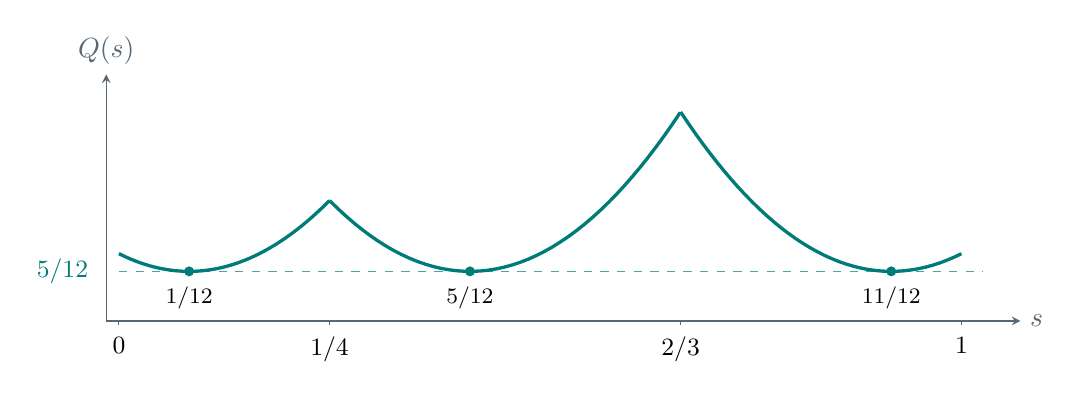
\begin{tikzpicture}[x=10.7cm,y=5.4cm,>=stealth]
 \draw[->,muted] (-.015,.30)--(1.07,.30) node[right]{$s$};
 \draw[->,muted] (-.015,.30)--(-.015,.88) node[above]{$Q(s)$};
 \draw[dashed,accent!70] (0,{5/12})--(1.025,{5/12});
 \draw[very thick,accent,domain=0:.25,samples=40]
   plot(\x,{5/12+6*(\x-1/12)^2});
 \draw[very thick,accent,domain=.25:.6666666667,samples=45]
   plot(\x,{5/12+6*(\x-5/12)^2});
 \draw[very thick,accent,domain=.6666666667:1,samples=40]
   plot(\x,{5/12+6*(\x-11/12)^2});
 \foreach \x/\lab in {0/0,.25/{1/4},.6666666667/{2/3},1/1}{
   \draw[muted] (\x,.30)--(\x,.29);
   \node[below,font=\small] at (\x,.285){$\lab$};}
 \node[left,font=\small,text=accent] at (-.025,{5/12}){$5/12$};
 \foreach \x/\lab in {.0833333333/{1/12},.4166666667/{5/12},.9166666667/{11/12}}{
   \fill[accent] (\x,{5/12}) circle(1.8pt);
   \node[below,font=\footnotesize] at (\x,.402){$\lab$};}
\end{tikzpicture}
\caption{An exact weighted deep hole. For $w=(1,2,3)$ and
$t=(1/2,1/4,-1/6)$, the event times are $0,1/4,2/3$.
All three quadratic branches have minimum $5/12$, at the marked
points. The mean is $W/12=1/2$, while the cubic jump correction is
$1/12$. The plot is of the exact piecewise quadratic formula.}
\label{r4:weightedfigure}
\end{figure}

There is also an exact nonnegative loss decomposition.  For the
fixed-phase functions in the proof of Theorem~\ref{r4c:cubic}, put
$G=Q-F^2/C$ away from events and $M=\min Q$.  Then
\begin{equation}\label{r4c:loss}
 M=B(a,q)-\frac1{C^2}\sum_e b_{j(e)}y_e^2
            -\int_0^1\bigl(G(s)-M\bigr)\,ds.
\end{equation}
The branch argument gives $G\geq M$, and
\eqref{r4c:loss} follows directly from
\eqref{r4c:meanQ}--\eqref{r4c:cubicbalance}.
Thus the exact radius is accompanied by two explicit nonnegative
losses for a prescribed point.

\subsection{One repeated frequency and balanced partitions}

Let $q=(k,1,\ldots,1)\in\Z^{d+1}$ and let its quadratic weights be
$(b,a_1,\ldots,a_d)$, where $k\geq1$, $d\geq1$, and all weights are
positive.  Write $A=\sum_i a_i$ and $C=k^2b+A$.  In the weighted
inner product, let $\pi_{a,q}$ be orthogonal projection onto
$q^\perp$ and let $\Lambda_{a,q}=\pi_{a,q}\Z^{d+1}$.
Since $q$ is an integer vector, its span is rational and this image
is a lattice.  More explicitly, a primitive integer vector spanning
the same line extends to an integer basis; the projections of the
remaining basis vectors form a lattice basis.  Its distance formula
is
\[
 \operatorname{dist}_{a}(\pi_{a,q}t,\Lambda_{a,q})^2
   =\min_s\left(b\|t_0+ks\|_{\Z}^2
                   +\sum_{i=1}^d a_i\|t_i+s\|_{\Z}^2\right).
\]

\begin{theorem}[Partition criterion for radius attainment]
\label{r4c:partition}
Define
\begin{equation}\label{r4c:partitionbound}
 B_2=\frac{b+A}{12}
       -\frac{k^4b^3+\sum_i a_i^3}{12(k^2b+A)^2}.
\end{equation}
Then $\rho(\Lambda_{a,q})^2\leq B_2$, with equality if and only if
$\{1,\ldots,d\}$ admits a partition into $k$ parts, each with
$a$-weight $A/k$.  If no such partition exists, the radius squared
is strictly less than $B_2$.

In particular, if $a_i=a$ for every $i$, then
\begin{equation}\label{r4c:equalweights}
 \rho(\Lambda_{a,q})^2
   =\frac{b+da}{12}
      -\frac{k^4b^3+da^3}{12(k^2b+da)^2}
 \quad\text{when }k\mid d,
\end{equation}
and the displayed expression is a strict upper bound when $k\nmid d$.
\end{theorem}

\begin{proof}
The bound is \eqref{r4c:generalbound}.  At equality, the $k$ events
of label $0$ have jump size $kb$ and spacing $1/k$.  The singleton
events between two consecutive such events form a part $I$.
Summing the centered-event gaps gives
\[
 \frac1k=\frac{kb+\sum_{i\in I}a_i}{C},
 \qquad\text{hence}\qquad
 \sum_{i\in I}a_i=\frac Ak.
\]
The $k$ intervals partition the singleton labels, proving necessity.

Conversely, choose a balanced partition, put a label $0$ between
successive parts, and order each part arbitrarily.  Assign the gaps
\eqref{r4c:eventgaps}.  Each interval between labels $0$ has length
$(kb+A/k)/C=1/k$.  A singleton label imposes no further restriction,
so Corollary~\ref{r4c:word} gives phases attaining the bound.
Finally, the maximum over phases exists by continuity on the compact
phase torus.  If a balanced partition does not exist, no maximum
equals $B_2$, proving strictness.  For equal $a_i$, balanced parts
exist exactly when $k$ divides $d$.
\end{proof}

\begin{remark}\label{r4c:complexity}
For positive integer input $a_i$, variable $k$, and $b=1$, deciding
whether \eqref{r4c:partitionbound} is attained is strongly
NP-complete.  A balanced partition is an NP certificate.  For
hardness, use the standard 3-PARTITION problem \cite{GJ}, with
$d=3k$, $\sum_i a_i=kB$, and $B/4<a_i<B/2$.  A part of weight $B$
must contain exactly three elements, so Theorem~\ref{r4c:partition}
is an exact reduction.  The rational threshold $B_2$ has polynomial
bit length.  This statement concerns attainment of one explicit
bound in the indicated family, represented by its integer parameters
and rational quadratic form; it is not a claim of a new general
hardness theorem for lattice covering radii.
\end{remark}

\section{The original prime-circle point and its missing bound}
\label{r4c:prime}

Let $p_n$ be the $n$th prime and use exactly the data of
\cite{PrimeCircles}:
\begin{align}
 \theta_n&=\sum_{p\leq p_n}\frac1p-\log\log p_n,
 & U_n&=e^{2\pi i\theta_n},\notag\\
 w_n&=p_{n+1}-p_{n-1},
 & W_N&=\sum_{n=2}^Nw_n=p_N+p_{N+1}-5,\label{r4c:primedata}\\
 M_N&=\sum_{n=2}^Nw_nU_n,
 & D_N&=W_N-|M_N|.\notag
\end{align}
For the weights and phases indexed by $2\leq n\leq N$, let
$\Lambda_N$ and $\pi_N$ be the objects in \eqref{r4c:lattice}, and set
\begin{equation}\label{r4c:primeQ}
 Q_N=\operatorname{dist}_{w}(\pi_N\theta,\Lambda_N)^2
    =\min_s\sum_{n=2}^Nw_n\|\theta_n+s\|_{\Z}^2.
\end{equation}
This changes neither the prime phases nor their weights.  The common
rotation is already present in the exact variational expression for
$D_N$.

\begin{corollary}[Exact bridge and growing worst case]
\label{r4c:primecorollary}
For every $N\geq2$,
\begin{equation}\label{r4c:primebridge}
 8Q_N\leq D_N\leq2\pi^2Q_N,
 \qquad
 \rho(\Lambda_N)^2
   =\frac{W_N}{12}
       -\frac{\sum_{n=2}^Nw_n^3}{12W_N^2}.
\end{equation}
Unconditionally, the prime number theorem implies
\begin{equation}\label{r4c:primegrowth}
 \rho(\Lambda_N)^2\sim\frac{W_N}{12}\sim\frac{p_N}{6}.
\end{equation}
The original prime-circle criterion of \cite{PrimeCircles},
reproved in Appendix~\ref{r4a:appendix}, gives
\begin{equation}\label{r4c:RHcriterion}
 \mathrm{RH}\quad\Longleftrightarrow\quad
 \sup_N Q_N<\infty.
\end{equation}
\end{corollary}

\begin{proof}
Proposition~\ref{r4c:bridge} and Theorem~\ref{r4c:radius} give
\eqref{r4c:primebridge}.  The prime number theorem gives
$p_{n+1}/p_n\to1$, hence $W_N\sim2p_N$ and $w_n/p_n\to0$.
For any $\varepsilon>0$, all sufficiently large $n$ satisfy
$w_n\leq\varepsilon p_n\leq\varepsilon p_N$ when $n\leq N$.
The finitely many remaining weights divided by $W_N$ tend to zero.
It follows that
\[
 \frac{\max_{2\leq n\leq N}w_n}{W_N}\longrightarrow0,
 \qquad
 \frac{\sum_{n=2}^Nw_n^3}{W_N^3}
 \leq\left(\frac{\max_{2\leq n\leq N}w_n}{W_N}\right)^2
 \longrightarrow0.
\]
This proves \eqref{r4c:primegrowth}.  Finally,
\eqref{r4c:primebridge} gives boundedness of $Q_N$ if and only if
$D_N$ is bounded.  Combining this with Theorem~\ref{r4a:criterion} gives \eqref{r4c:RHcriterion}.
\end{proof}

The missing arithmetic statement is the bounded distance of the
\emph{prescribed prime point}, $Q_N=O(1)$.  The phase-uniform
covering problem has a different answer: its exact squared radius
grows like $p_N/6$.  Thus no bound depending only on these weights
and valid for all phase vectors can provide the required constant.
This is a sharp obstruction to that uniform route, not an
obstruction to using additional arithmetic information about
$\theta_n$.  Neither \eqref{r4c:primebridge} nor the radius formula
proves boundedness in \eqref{r4c:RHcriterion}.

\section{Sharp finite-polygon approximation}
\label{r4c:polygon}

A regular polygon approximation can preserve the original complex
sum exactly while discretizing only the direction in which its
support is evaluated.  For an integer $k\geq2$ and an orientation
$\eta\in\R$, define
\begin{equation}\label{r4c:polygondef}
 D_{N,k,\eta}
 =W_N-\max_{0\leq j<k}
     \Re\!\left(e^{-i(\eta+2\pi j/k)}M_N\right).
\end{equation}
In particular, this does not replace $U_n$ by polygon vertices.

\begin{proposition}[Exact support error]\label{r4c:polygonerror}
If $M_N\ne0$, let $\delta$ be the circular distance of $\arg M_N$
from the grid $\eta+(2\pi/k)\Z$, so $0\leq\delta\leq\pi/k$.
Then
\begin{equation}\label{r4c:exacterror}
 D_{N,k,\eta}-D_N=|M_N|(1-\cos\delta).
\end{equation}
If $M_N=0$, the difference is zero.  In all cases,
\begin{equation}\label{r4c:polygonbound}
 0\leq D_{N,k,\eta}-D_N
   \leq W_N\bigl(1-\cos(\pi/k)\bigr)
   \leq\frac{\pi^2W_N}{2k^2}.
\end{equation}
For arbitrary phases with the given positive weights, the first
upper bound is attained.  Consequently the optimal phase-uniform
error is exactly $W_N(1-\cos(\pi/k))$, and a sequence of such errors
is bounded if and only if $W_N/k_N^2=O(1)$.
\end{proposition}

\begin{proof}
The largest grid projection of $M_N$ is $|M_N|\cos\delta$, giving
\eqref{r4c:exacterror}.  Since $|M_N|\leq W_N$, the upper bounds
follow from $1-\cos x\leq x^2/2$.
To attain the first bound, take all phases equal to a direction
halfway between adjacent grid directions.  Then $|M_N|=W_N$ and
$\delta=\pi/k$.  Finally,
\[
 \frac{2}{k^2}\leq1-\cos(\pi/k)
       \leq\frac{\pi^2}{2k^2}
\]
for $k\geq2$, proving the asserted necessary and sufficient scale
for the phase-uniform error.
\end{proof}

For any orientations $\eta_N$ and meshes satisfying
$W_N/k_N^2=O(1)$, Proposition~\ref{r4c:polygonerror} gives
\begin{equation}\label{r4c:polygoncriterion}
 \sup_ND_{N,k_N,\eta_N}<\infty
 \quad\Longleftrightarrow\quad
 \sup_ND_N<\infty.
\end{equation}
Thus $k_N$ on the order of $\sqrt{W_N}$ gives a controlled finite
polygon version of the original criterion.  Optimality of that
scale is a statement uniform over phases, not a lower bound on the
mesh required for the specific prime sequence.

For comparison, a fixed grid can introduce a spurious error of
order $W_N$.  The prime reciprocal asymptotic in
\cite{PrimeCircles} gives $U_n\to U_\infty=e^{2\pi i B_{\mathbb P}}$,
and weighted Cesaro convergence gives $M_N/W_N\to U_\infty$.
If $U_\infty$ is not a direction of a fixed grid, then
\[
 \frac{D_{N,k,\eta}-D_N}{W_N}
 \longrightarrow
 1-\cos\operatorname{dist}_{\R/(2\pi\Z)}
       \bigl(\arg U_\infty,\eta+(2\pi/k)\Z\bigr)>0.
\]
No irrationality assertion about $B_{\mathbb P}$ is needed: the
statement is explicitly conditional on grid alignment.  Conversely,
choosing the grid orientation after seeing $M_N$ can make the
approximation error zero, but then supplies no new estimate for
$D_N$ itself.

\section{Li curvature and exact regular-polygon certificates}
\label{r4l:section}

The Cayley geometry of the zeros and Li's positivity criterion are
classical \cite{Li,Lagarias,Suzuki}.  The corrected-Li square-summability
criterion in \cite{PrimeCircles} is a different construction from the
one below.  We use the ordinary Li coefficients, take their second
differences, and transport the resulting quadratic forms to regular
polygons by exact finite Fourier identities.  The infinite positivity
condition remains equivalent to the Riemann hypothesis.  What can be
proved here is an explicit finite obstruction from any hypothetical
off-line zero, including control of all omitted zeros, and an explicit
countermodel showing why an arbitrary fixed number of positive tests
does not suffice.

\subsection{An absolutely convergent sequence and its generating function}

Use the normalization
\[
 \xi(s)=\tfrac12s(s-1)\pi^{-s/2}\Gamma(s/2)\zeta(s),
 \qquad \xi(1)=\tfrac12,
\]
and the ordinary Li coefficients
\begin{equation}\label{r4l:lidef}
 \lambda_n=\frac1{(n-1)!}
 \left.\frac{d^n}{ds^n}
     \bigl(s^{n-1}\log\xi(s)\bigr)\right|_{s=1},
 \qquad n\ge1.
\end{equation}
Extend them by $\lambda_0=0$ and $\lambda_{-n}=\lambda_n$.
Zeros in a sum are counted with their multiplicities unless we explicitly
form a set of distinct zeros.  Put
\begin{equation}\label{r4l:cayley}
 u_\rho=1-\frac1\rho,
 \qquad w_\rho=\frac1{\rho(1-\rho)},
 \qquad a_n=\lambda_{n+1}-2\lambda_n+\lambda_{n-1}
 \quad(n\in\Z).
\end{equation}
The usual zero symmetries imply
\[
 u_{1-\rho}=u_\rho^{-1},\qquad
 u_{1-\bar\rho}=1/\bar u_\rho,\qquad
 w_{1-\bar\rho}=\bar w_\rho.
\]
Also $|u_\rho|=1$ exactly when $\Re\rho=1/2$.

\begin{lemma}[Curvature normalization]\label{r4l:curvature}
The sequence $(a_n)_{n\in\Z}$ is real and even, and
\begin{equation}\label{r4l:zeromoments}
 a_n=\sum_\rho w_\rho u_\rho^n
 \qquad(n\in\Z),
\end{equation}
with absolute convergence for every fixed $n$.  In particular,
\[
 a_0=2\lambda_1=2+\gamma_E-\log(4\pi)>0.
\]
As an identity of holomorphic germs at zero,
\begin{equation}\label{r4l:generating}
 \mathcal A(z):=\sum_{n\ge0}a_nz^n
 =\lambda_1+\frac{\xi'}{\xi}\!\left(\frac1{1-z}\right).
\end{equation}
\end{lemma}
\begin{proof}
The classical zero formula is
\[
 \lambda_n=\lim_{T\to\infty}
 \sum_{|\Im\rho|\le T}(1-u_\rho^n).
\]
The same convention holds at negative integers; replacing $\rho$ by
$1-\rho$ proves evenness, and conjugation proves reality.  Taking a
second difference of the finite sums gives
\[
 -u_\rho^{n-1}(u_\rho-1)^2
 =(2-u_\rho-u_\rho^{-1})u_\rho^n
 =w_\rho u_\rho^n.
\]
For fixed $n$, this is $O_n(|\Im\rho|^{-2})$ on the tail.  The
standard zero-count estimate $N(T)=O(T\log T)$ proves absolute
convergence, so the second differences pass to the limit.

Let $s(z)=1/(1-z)$ and
$L(z)=\log(2\xi(s(z)))$, with its normalized branch near zero.
The Leibniz rule in \eqref{r4l:lidef}, or finite Taylor substitution,
gives
\[
 [z^n]L(z)
 =\sum_{j=1}^n\binom{n-1}{j-1}
       \frac{(\log\xi)^{(j)}(1)}{j!}
 =\frac{\lambda_n}{n}.
\]
Thus the second-difference definition, including $a_0=2\lambda_1$,
yields
\[
 \mathcal A(z)=\lambda_1+(1-z)^2L'(z)
 =\lambda_1+\frac{\xi'}{\xi}(s(z)).
\]
The stated value of $a_0$ is the usual evaluation of
$2(\xi'/\xi)(1)$.
\end{proof}

\subsection{Circle energies and finite quadratic forms}

Set
\[
 T_N=(a_{k-j})_{j,k=0}^N,
 \qquad p(z)=\sum_{j=0}^Nc_jz^j,
 \qquad Q(p)=c^*T_Nc.
\]
The choice $a_{k-j}$ fixes the conjugation convention.  Since $a_n$ is
real and even, it agrees with $a_{j-k}$ here.  Absolute convergence in
Lemma~\ref{r4l:curvature} gives the unconditional identity
\begin{equation}\label{r4l:quadratic}
 Q(p)=\sum_\rho w_\rho p(u_\rho)
                    \overline{p(1/\bar u_\rho)}.
\end{equation}

\begin{proposition}[Classical positivity in curvature coordinates]
\label{r4l:equivalence}
The following statements are equivalent:
\begin{enumerate}
\item The Riemann hypothesis holds.
\item $T_N$ is positive semidefinite for every $N\ge0$.
\item $|a_n|\le a_0$ for every $n\ge1$.
\end{enumerate}
Under these conditions the measure
\begin{equation}\label{r4l:measure}
 \nu=\sum_\rho\frac{\delta_{u_\rho}}{1/4+(\Im\rho)^2}
\end{equation}
is a finite positive measure on the unit circle, with mass $a_0$, and
\begin{equation}\label{r4l:energy}
 Q(p)=\int|p(u)|^2\,d\nu(u),
 \qquad
 \lambda_n=\frac12\int|1+u+\cdots+u^{n-1}|^2\,d\nu(u).
\end{equation}
\end{proposition}
\begin{proof}
Under the Riemann hypothesis, $|u_\rho|=1$ and
\[
 w_\rho=|1-u_\rho|^2
       =\frac1{1/4+(\Im\rho)^2}>0.
\]
Consequently \eqref{r4l:zeromoments} is a Fourier-moment representation
by \eqref{r4l:measure}, and \eqref{r4l:quadratic} gives the first
identity in \eqref{r4l:energy}.  Taking all $c_j=1$, or telescoping
second differences, gives
\[
 (1,\ldots,1)T_{n-1}(1,\ldots,1)^t
 =na_0+2\sum_{j=1}^{n-1}(n-j)a_j=2\lambda_n.
\]
This proves the second identity and the first implication.

The principal submatrix of $T_n$ on indices $0,n$ is
\[
 \begin{pmatrix}a_0&a_n\\a_n&a_0\end{pmatrix}.
\]
Its positivity implies $|a_n|\le a_0$, proving the second implication.
If all these bounds hold, $\mathcal A$ is holomorphic throughout the
unit disk.  A zero $\rho$ with $\Re\rho>1/2$ would give a pole of
$(\xi'/\xi)(s(z))$ at $z=u_\rho$ inside that disk.  This pole is
nonremovable: its multiplicity is positive and $s'(u_\rho)\ne0$.
Meromorphic continuation of \eqref{r4l:generating} excludes it.  The
functional equation then excludes zeros to the left of $1/2$ as well.
\end{proof}

\begin{remark}[Attribution and the remaining positivity problem]
\label{r4l:classicalscope}
The identity
\[
 a_0+2\sum_{n\ge1}a_nz^n
 =2\frac{\xi'}{\xi}\!\left(\frac1{1-z}\right)
\]
identifies this proposition with the disk form of the classical
positive-real logarithmic-derivative criterion \cite{Lagarias}.
Li's criterion and its connections with Weil positivity and norm
identities are established results \cite{Li,Suzuki}.  The proposition
does not prove that its matrices are positive.  The $2$-by-$2$ tests
range over every separation $n$, not merely adjacent matrix entries.
\end{remark}

\subsection{Exact finite polygons and their signed mass}

For $M\ge1$ put
\begin{align}
 F_M(\theta)&=a_0+2\sum_{n=1}^M
      \left(1-\frac n{M+1}\right)a_n\cos(n\theta),
       \label{r4l:fejer}\\
 q_M&=2M+1,\qquad \theta_{M,j}=\frac{2\pi j}{q_M},
 \qquad
 \eta_{M,j}=\frac{F_M(\theta_{M,j})}{q_M}
 \quad(0\le j<q_M).\label{r4l:polygonweights}
\end{align}
These are unconditional, possibly signed, weights at the vertices of
a regular $(2M+1)$-gon.  They do not assume that the actual zero images
are roots of unity.

\begin{theorem}[Exact polygon transport]\label{r4l:polygon}
For every $M\ge1$,
\begin{equation}\label{r4l:polygonmoments}
 \sum_j\eta_{M,j}=a_0,
 \qquad
 \sum_j\eta_{M,j}e^{in\theta_{M,j}}
 =\left(1-\frac{|n|}{M+1}\right)a_n
 \quad(|n|\le M).
\end{equation}
The Riemann hypothesis is equivalent to
$\eta_{M,j}\ge0$ for every $M$ and $j$.
\end{theorem}
\begin{proof}
Expand \eqref{r4l:fejer} in exponentials and use finite Fourier
orthogonality.  For $|n|\le M$, all unwanted frequencies have absolute
value at most $2M<q_M$, so there is no aliasing.  This proves
\eqref{r4l:polygonmoments}.

Under the Riemann hypothesis, $F_M$ is the convolution of the positive
measure \eqref{r4l:measure} with the Fejer kernel
\[
 \frac1{M+1}|1+e^{i\theta}+\cdots+e^{iM\theta}|^2,
\]
so all the vertex weights are nonnegative.  Conversely, fix a
polynomial $p(z)=\sum_{k=0}^Nc_kz^k$.  For $M\ge N$, the exact
moment identities give
\begin{equation}\label{r4l:polygonquadratic}
 \sum_{j=0}^{q_M-1}\eta_{M,j}|p(e^{i\theta_{M,j}})|^2
 =\sum_{j,k=0}^N\bar c_jc_k
       \left(1-\frac{|k-j|}{M+1}\right)a_{k-j}.
\end{equation}
If all weights are nonnegative, the left side is nonnegative.  Letting
$M\to\infty$ gives $Q(p)\ge0$.  Proposition~\ref{r4l:equivalence}
then proves the Riemann hypothesis.
\end{proof}

\begin{corollary}[A finite polygon from a negative certificate]
\label{r4l:negativepolygon}
Suppose $p(z)=\sum_{k=0}^Nc_kz^k$ satisfies $Q(p)=-\varepsilon<0$,
and define
\[
 E(p)=\sum_{j,k=0}^N|k-j|\,|c_j|\,|c_k|\,|a_{k-j}|.
\]
For every $M\ge N$ with $M+1>E(p)/\varepsilon$, at least one
$\eta_{M,j}$ is negative.
\end{corollary}
\begin{proof}
The right side of \eqref{r4l:polygonquadratic} differs from $Q(p)$
by at most $E(p)/(M+1)$, so it is negative.  A sum with nonnegative
weights and nonnegative summands could not be negative.
\end{proof}

\begin{proposition}[The exponential size of a polygon obstruction]
\label{r4l:polygongrowth}
Put
\[
 V_M=\sum_j|\eta_{M,j}|,
 \qquad
 R=\min\left\{1,
       \inf_{\substack{\xi(\rho)=0\\\Re\rho>1/2}}
                \left|1-\frac1\rho\right|\right\},
\]
where the infimum of the empty set is $+\infty$.  Then
\begin{equation}\label{r4l:growthrate}
 \limsup_{M\to\infty}V_M^{1/M}=R^{-1}.
\end{equation}
Under the Riemann hypothesis, $V_M=a_0$ for every $M$.  If it fails,
then $R<1$, and the total negative vertex mass
\[
 N_M^-:=\sum_j\max\{-\eta_{M,j},0\}
       =\frac{V_M-a_0}{2}
\]
has the same exponential limsup rate $R^{-1}>1$.
\end{proposition}
\begin{proof}
Equation~\eqref{r4l:generating} shows that the Taylor radius of
$\mathcal A$ is exactly $R$.  If an off-line zero exists, its symmetry
partner on the right of $1/2$ gives a pole inside the disk.  Zeros of
large height have $|1-1/\rho|\to1$, so the smallest modulus strictly
below one is attained, and no pole there can cancel.  If no off-line
zero exists, the function is holomorphic in the disk and has poles
at the unit-circle images of its zeros.  Thus its radius is one.
Cauchy--Hadamard gives
\[
 \limsup_{n\to\infty}|a_n|^{1/n}=R^{-1}.
\]
From \eqref{r4l:polygonmoments} with $n=M$, and from the triangle
inequality in \eqref{r4l:fejer}, respectively,
\[
 \frac{|a_M|}{M+1}\le V_M
 \le a_0+2\sum_{n=1}^M|a_n|.
\]
These inequalities give \eqref{r4l:growthrate}.  The total signed
mass is always $a_0$, so the formula for $N_M^-$ is exact.  If the
exponential limsup is greater than one, subtracting the fixed number
$a_0$ and dividing by two does not change it.
\end{proof}

\subsection{Finite zero sets and their exact inertia}

The next statement concerns a finite truncation only.  Its proof also
explains which negative direction the infinite-tail argument must
preserve.

\begin{proposition}[Finite-truncation inertia]\label{r4l:inertia}
Let $Z$ be a finite set of distinct nodes $u\in\C\setminus\{0,1\}$,
closed under $u\mapsto u^*=1/\bar u$, with positive multiplicities
$m_u=m_{u^*}$.  Put
\[
 w(u)=2-u-u^{-1},\qquad
 a_n^Z=\sum_{u\in Z}m_uw(u)u^n.
\]
Let $U$ be the number of nodes on the unit circle and $P$ the number
of off-circle pairs $\{u,u^*\}$, so $r=|Z|=U+2P$.  For $N\ge r-1$,
the Hermitian matrix $(a_{k-j}^Z)_{j,k=0}^N$ has inertia
\begin{equation}\label{r4l:inertiaeq}
 (n_+,n_-,n_0)=(U+P,P,N+1-r).
\end{equation}
\end{proposition}
\begin{proof}
For a polynomial $p$ the form is
\[
 \sum_{u\in Z}m_uw(u)p(u)\overline{p(u^*)}.
\]
At a unit-circle node $u=u^*$, its coefficient
$m_u(2-2\Re u)$ is strictly positive.  Each off-circle pair contributes
a $2$-by-$2$ Hermitian block with zero diagonal and off-diagonal
entries $m_uw(u)$ and its conjugate.  Its eigenvalues are
$m_u|w(u)|$ and $-m_u|w(u)|$.

Evaluation at the $r$ distinct nodes is an isomorphism on polynomials
of degree at most $r-1$, by the Vandermonde determinant.  Sylvester's
law of inertia therefore gives \eqref{r4l:inertiaeq} at $N=r-1$.
For larger $N$ evaluation remains surjective and its kernel has
dimension $N+1-r$, supplying the zero directions.  Multiplicity
changes the scale of a block, not its dimension or its signs.
\end{proof}

\subsection{A finite negative certificate with the full tail controlled}

\begin{theorem}[An explicit obstruction from an off-line zero]
\label{r4l:offzero}
Suppose $\rho_0$ is a nontrivial zero with $\Re\rho_0\ne1/2$.
Set
\[
 u=1-\rho_0^{-1},\quad v=1/\bar u,
 \quad w_0=[\rho_0(1-\rho_0)]^{-1},
 \quad m_0=\operatorname{mult}(\rho_0),
\]
and choose
\[
 T>H:=\max\{|\rho_0|,|1-\bar\rho_0|\}.
\]
Let $Z_T$ be the set of distinct Cayley nodes of all zeros with
$|\Im\rho|\le T$, let $r=|Z_T|$, and define
\begin{align*}
 L_a(z)&=\prod_{b\in Z_T\setminus\{a\}}\frac{z-b}{a-b},\qquad
 K_a(T)=\prod_{b\in Z_T\setminus\{a\}}
             \frac{|1-b|+T^{-1}}{|a-b|},\\
 K&=K_u(T)+K_v(T),\qquad
 B_T=(1+4/T^2)\frac{\xi'}{\xi}(2).
\end{align*}
For any integer $L\ge0$ put
\begin{equation}\label{r4l:filter}
 p_L(z)=\left(\frac{1-z}{1-u}\right)^L L_u(z)
       -\frac{w_0}{|w_0|}
        \left(\frac{1-z}{1-v}\right)^L L_v(z).
\end{equation}
Then $\deg p_L\le r-1+L$ and
\begin{equation}\label{r4l:tailcertificate}
 Q(p_L)\le -2m_0|w_0|+K^2B_T(H/T)^{2L}.
\end{equation}
In particular, any $L\ge0$ satisfying
\begin{equation}\label{r4l:Lchoice}
 K^2B_T(H/T)^{2L}<m_0|w_0|
\end{equation}
gives a finite negative quadratic-form certificate and, by
Corollary~\ref{r4l:negativepolygon}, a finite regular polygon with a
negative arithmetic vertex weight.
\end{theorem}
\begin{proof}
The set $Z_T$ is finite and closed under $a\mapsto1/\bar a$, and it
contains the distinct nodes $u,v$.  By interpolation,
\[
 p_L(u)=1,\qquad p_L(v)=-w_0/|w_0|,
 \qquad p_L(a)=0\quad(a\in Z_T\setminus\{u,v\}).
\]
The multiplicities at $u$ and $v$ agree.  Their contribution to
\eqref{r4l:quadratic} is exactly
\[
 m_0\left(w_0\overline{-w_0/|w_0|}
           +\bar w_0(-w_0/|w_0|)\right)
 =-2m_0|w_0|.
\]
All other low-zero terms vanish.

For the tail, the conjugate-paired Hadamard product gives
\begin{equation}\label{r4l:A2}
 \frac{\xi'}{\xi}(2)
 =\sum_\rho\Re\frac1{2-\rho}
 =\frac32-\frac{\gamma_E+\log\pi}{2}
                 +\frac{\zeta'}{\zeta}(2)>0.
\end{equation}
Every term of the real-part sum is positive.  If
$\rho=\beta+i\gamma$ lies in the critical strip and $|\gamma|>T$, then
\[
 |w_\rho|\le\frac1{\gamma^2}
 \le\frac{1+4/T^2}{4+\gamma^2}
 \le(1+4/T^2)\Re\frac1{2-\rho}.
\]
Indeed $1<2-\beta<2$, so the final real part is at least
$1/(4+\gamma^2)$.  Summing proves
\[
 \sum_{|\Im\rho|>T}|w_\rho|\le B_T.
\]
This bound uses no assumption on the horizontal positions of tail
zeros beyond the unconditional critical strip.

Both nodes $u_\rho$ and $1/\bar u_\rho$ of a tail pair lie in the
disk $|z-1|<1/T$.  On that disk $|L_a(z)|\le K_a(T)$, and
\[
 \left|\frac{1-z}{1-u}\right|,
 \ \left|\frac{1-z}{1-v}\right|\le H/T.
\]
Therefore both polynomial values in a tail term of
\eqref{r4l:quadratic} have modulus at most $K(H/T)^L$.  Their total
absolute contribution is at most $K^2B_T(H/T)^{2L}$, proving
\eqref{r4l:tailcertificate}.  Since $H/T<1$, a finite $L$ satisfying
\eqref{r4l:Lchoice} exists.
\end{proof}

\begin{remark}[Degree, completeness, and an optional sharper budget]
\label{r4l:certificatescope}
An explicit admissible choice in Theorem~\ref{r4l:offzero} is
\[
 L=\max\left\{0,
 1+\left\lfloor
 \frac{\log(K^2B_T/(m_0|w_0|))}{2\log(T/H)}
 \right\rfloor\right\}.
\]
The negativity margin is greater than $m_0|w_0|$.  Once the coefficients
of $p_L$ are formed, the finite number $E(p_L)$ in
Corollary~\ref{r4l:negativepolygon} gives an explicit sufficient polygon
size.  No efficiency is claimed: close low zeros can make the
Lagrange constants very large.

The low set must contain \emph{all} zeros up to height $T$, with their
multiplicities.  A chosen subset would not justify discarding the
other low-zero contributions.  Complex coefficients in $p_L$ are
allowed; since $T_N$ is real symmetric, at least one of its real and
imaginary coefficient vectors also has a negative quadratic form.
If the complete low-zero data are available, $B_T$ can be replaced by
the sharper nonnegative budget
\[
 (1+4/T^2)\left(
 \frac{\xi'}{\xi}(2)-
 \sum_{|\Im\rho|\le T}\Re\frac1{2-\rho}\right).
\]
The result is conditional on an off-line zero; it neither exhibits
such a zero nor proves positivity for the actual infinite sequence.
\end{remark}

\subsection{An explicit limitation of every fixed finite cutoff}

\begin{proposition}[Positive finite tests with an off-line quartet]
\label{r4l:finitecountermodel}
For every $N\ge1$ there is a finite zero multiset, closed under
conjugation and $\rho\mapsto1-\rho$, with zeros off the critical line,
whose curvature matrix $T_N$ is strictly positive definite.  All its
polygon tests of orders $M\le N$ are strictly positive at every angle.
The multiset is the zero set of a real polynomial satisfying
$P(s)=P(1-s)$ after normalization.
\end{proposition}
\begin{proof}
Choose an odd integer $m\ge N+2$ and begin with the Cayley nodes
\[
 u_j=e^{2\pi i j/m},\qquad 1\le j<m.
\]
Their inverse Cayley images $(1-u_j)^{-1}$ are nonreal, lie on the
critical line, and have both required symmetries.  Summing
$(2-u-u^{-1})u^n$ over the roots of unity gives, for $0\le n\le N$,
\[
 a_0^{(0)}=2m,\qquad a_1^{(0)}=-m,\qquad
 a_n^{(0)}=0\quad(2\le n\le N).
\]
The term at $u=1$ would have zero weight and can be inserted in this
calculation.  The condition $m\ge N+2$ excludes the other cyclic
aliases.  Thus $T_N^{(0)}$ is $m$ times the tridiagonal matrix with
diagonal $2$ and adjacent diagonals $-1$, whose least eigenvalue is
\begin{equation}\label{r4l:countermodelmargin}
 \ell_N=2m\left(1-\cos\frac\pi{N+2}\right)
 \ge\frac{4m}{(N+2)^2}\ge\frac4{N+2}.
\end{equation}

Add the off-line quartet
\[
 \tfrac14\pm iT,\qquad\tfrac34\pm iT,
 \qquad T=2(N+2).
\]
For each of these zeros, $|w_\rho|\le T^{-2}$ and
\[
 \max\{|u_\rho|,|u_\rho|^{-1}\}
 \le(1+T^{-2})^{1/2}.
\]
Hence every entry of the perturbation of $T_N$ has absolute value at
most $4T^{-2}(1+T^{-2})^{N/2}$.  Its operator norm is at most
\begin{equation}\label{r4l:countermodelperturbation}
 4(N+1)T^{-2}(1+T^{-2})^{N/2}
 \le\frac{\mathrm e(N+1)}{(N+2)^2}
 <\frac4{N+2}.
\end{equation}
Equations~\eqref{r4l:countermodelmargin} and
\eqref{r4l:countermodelperturbation} prove strict positivity of the
perturbed $T_N$.  Its smaller $T_M$ are positive principal submatrices.
For $v_M(\theta)=(1,e^{i\theta},\ldots,e^{iM\theta})^t$,
\[
 F_M(\theta)=\frac1{M+1}v_M(\theta)^*T_Mv_M(\theta)>0,
\]
which proves every asserted finite polygon test.

The full zero multiset has even size and the two stated symmetries.
The product of its linear factors is therefore real and invariant
under $s\mapsto1-s$; normalization at zero preserves that identity.
\end{proof}

\begin{remark}[The exact role of the positive-weight flow]
\label{r4l:flowgap}
The polygon vertices form a finite cyclic group, and
\eqref{r4l:polygonmoments}--\eqref{r4l:polygonquadratic} are exact
periodic identities.  This is a valid bridge to the finite-periodic
framework of the lattice-covering flow.  But that flow theorem
assumes positive weights.  For the arithmetic weights
\eqref{r4l:polygonweights}, proving this hypothesis at every order
is already equivalent to the Riemann hypothesis.  Applying the
positive-weight theorem before establishing those signs would be
circular.  Replacing the weights by absolute values would change the
moments and the original quadratic forms.

Proposition~\ref{r4l:finitecountermodel} is a countermodel to an
inference from a fixed finite collection of tests and the functional
symmetries.  It is not a counterexample to the Riemann hypothesis:
the polynomial does not have the Euler product or the actual zeta
coefficients.  The remaining arithmetic task is to prove positivity
uniformly in degree for the actual sequence.  The finite transport,
inertia calculation, and tail-controlled certificate above do not
establish that uniform positivity, and no claim of historical
priority for these consequences of classical methods is made.
\end{remark}

% Manuscript fragment. No preamble, document environment, or bibliography.
% Bibliography keys: BaezDuarte, Balazard, Burnol, MaierRassias, VMRC200.
% All internal labels have prefix r4n:.
% The optional five-cell calculation is isolated in a remark.

\section{Nyman--Beurling approximation as a signed residue flow}
\label{r4n:sec-nyman}

The fractional-part functions in the Nyman--Beurling criterion can be
written exactly as finite periodic flows of the form used in
\cite{VMRC200}.  The relevant flow has signed coefficients and zero
continuous slope.  We make that distinction explicit, give a finite
formula for its full approximation norm, and determine a sharp local
obstruction to replacing the signed coefficients by nonnegative ones.
The strong criterion and the underlying biorthogonal construction
are established results; the calculations below do not constitute a
proof of the Riemann hypothesis.

\subsection{The established strong criterion and tail cancellation}
\label{r4n:subsec-criterion}

Write $\chi=1_{(0,1)}$ and
\[
 e_n(x)=\left\{\frac1{nx}\right\}\quad(x>0,\ n\ge1).
\]
The strong discrete Nyman--Beurling theorem of B\'aez-Duarte
\cite{BaezDuarte} states that
\begin{equation}
\label{r4n:eq-strong-bd}
 \mathrm{RH}
 \quad\Longleftrightarrow\quad
 \chi\in\overline{\operatorname{span}\{e_n:n\ge1\}}^{\,L^2(0,\infty)}.
\end{equation}
For $n\ge2$, define the tail-cancelled generators
\begin{equation}
\label{r4n:eq-generators}
 f_n(x)=e_n(x)-\frac1n e_1(x).
\end{equation}
They vanish for $x>1$.
For $N\ge2$, set
\[
 \begin{aligned}
 d_N&=\inf_{a\in\R^N}
       \left\|\chi-\sum_{n=1}^Na_ne_n\right\|_{L^2(0,\infty)},\\
 \delta_N&=\inf_{c\in\R^{N-1}}
       \left\|1-\sum_{n=2}^Nc_nf_n\right\|_{L^2(0,1)}.
 \end{aligned}
\]
Real coefficients suffice, since taking real parts does not increase
the distance from a real target.

We will use the elementary comparison
\begin{equation}
\label{r4n:eq-distance-comparison}
 d_N\le\delta_N\le(1+\sqrt2)d_N.
\end{equation}
The first inequality follows because every $f_n$ is a combination of
$e_n$ and $e_1$.  To prove the second, let
$h=\sum_{n=1}^Na_ne_n$ have error $\varepsilon$, and put
$A=\sum_{n=1}^Na_n/n$.  On $x>1$, one has $h(x)=A/x$.
Thus the squared error on that interval is $A^2$, and $|A|\le\varepsilon$.
Moreover,
\[
 h-Ae_1=\sum_{n=2}^Na_nf_n,\qquad
 \|\chi-(h-Ae_1)\|_2\le(1+\|e_1\|_2)\varepsilon.
\]
The bounds $e_1(x)\le1$ on $(0,1)$ and $e_1(x)=1/x$ on $(1,\infty)$
give $\|e_1\|_2\le\sqrt2$.
Taking infima proves \eqref{r4n:eq-distance-comparison}, and therefore
\begin{equation}
\label{r4n:eq-anchored-criterion}
 \mathrm{RH}\quad\Longleftrightarrow\quad\delta_N\longrightarrow0.
\end{equation}
This is a reduction of the cited strong criterion, not an independent
proof of that criterion.

\subsection{An exact finite orbit and its Gram matrix}
\label{r4n:subsec-finite}

For $u>0$ and $k=\lfloor u\rfloor$, cancellation of the fractional
linear parts gives
\begin{equation}
\label{r4n:eq-residue-values}
 f_n(1/u)=\{u/n\}-\{u\}/n=\frac{k\bmod n}{n}.
\end{equation}
In particular, each $f_n$ is a nonnegative step function.
The step-space norm and its relation to these generators are part of
the Vasyunin--Balazard framework \cite[Sections~1--2]{Balazard}.

\begin{theorem}[Exact finite residue formula]
\label{r4n:thm-finite-gram}
Fix $N\ge2$ and set $L=\operatorname{lcm}(1,\ldots,N)$.
For $c=(c_2,\ldots,c_N)\in\R^{N-1}$, put
\[
 g=\sum_{n=2}^Nc_nf_n,\qquad
 z_k=\sum_{n=2}^Nc_n\frac{k\bmod n}{n}.
\]
Define positive weights
\begin{equation}
\label{r4n:eq-orbit-weights}
 W_{L,r}=\sum_{m=0}^{\infty}
       \frac1{(mL+r)(mL+r+1)}
       \qquad(1\le r\le L).
\end{equation}
Then $\sum_{r=1}^LW_{L,r}=1$ and
\begin{equation}
\label{r4n:eq-finite-error}
 E(c):=\|1-g\|_{L^2(0,1)}^2
      =\sum_{r=1}^{L}W_{L,r}|1-z_r|^2.
\end{equation}
Let
\[
 \begin{aligned}
 V_{r,n}&=\frac{r\bmod n}{n},
 &W&=\operatorname{diag}(W_{L,1},\ldots,W_{L,L}),\\
 G_N&=V^{\mathsf T}WV,
 &b_N&=V^{\mathsf T}W\mathbf1,
 \end{aligned}
\]
where $1\le r\le L$ and $2\le n\le N$.
The matrix $G_N$ is positive definite, and
\begin{equation}
\label{r4n:eq-gram-distance}
 \begin{aligned}
 c^*&=G_N^{-1}b_N,\\
 \delta_N^2&=1-b_N^{\mathsf T}G_N^{-1}b_N
 =\frac{\det\begin{pmatrix}1&b_N^{\mathsf T}\\b_N&G_N\end{pmatrix}}
        {\det G_N}.
 \end{aligned}
\end{equation}
Consequently \eqref{r4n:eq-anchored-criterion} is equivalent to
$b_N^{\mathsf T}G_N^{-1}b_N\to1$.
\end{theorem}

\begin{proof}
On $I_k=(1/(k+1),1/k)$, equation
\eqref{r4n:eq-residue-values} gives $g(x)=z_k$.
Since $|I_k|=1/[k(k+1)]$,
\begin{equation}
\label{r4n:eq-step-norm}
 E(c)=\sum_{k=1}^{\infty}\frac{|1-z_k|^2}{k(k+1)}.
\end{equation}
All endpoints have measure zero.  The sequence $z_k$ is $L$-periodic.
Grouping the nonnegative terms by their residues modulo $L$ proves
\eqref{r4n:eq-finite-error}.  Applying the same grouping to
$\sum_{k\ge1}1/[k(k+1)]=1$ proves that the weights sum to one.

Expansion of \eqref{r4n:eq-finite-error} gives
\[
 E(c)=1-2b_N^{\mathsf T}c+c^{\mathsf T}G_Nc.
\]
To prove positive definiteness, suppose $Vc=0$.
Periodicity implies $z_k=0$ for all $k\ge0$.
Writing $A=\sum_{n=2}^Nc_n/n$, one has
\begin{equation}
\label{r4n:eq-first-difference}
 z_k=Ak-\sum_{n=2}^k c_n\lfloor k/n\rfloor,\qquad
 z_k-z_{k-1}=A-\sum_{\substack{n\mid k\\n\ge2}}c_n,
\end{equation}
with coefficients outside the given support set to zero.
The equality $z_1=0$ gives $A=0$; induction on $k=2,\ldots,N$
in the second identity then gives $c_k=0$.
Since every weight is positive, $G_N$ is positive definite.
Completing the square yields the minimizer and the first distance
formula in \eqref{r4n:eq-gram-distance}.
The block determinant identity gives the second formula.
The asserted equivalence now follows from
\eqref{r4n:eq-anchored-criterion}.
\end{proof}

The orbit weights can, if desired, be evaluated by
\begin{equation}
\label{r4n:eq-digamma}
 W_{L,r}=\frac1L\left[
       \psi\left(\frac{r+1}{L}\right)
       -\psi\left(\frac rL\right)\right],
 \qquad \psi=\Gamma'/\Gamma.
\end{equation}
Indeed, write $1/[k(k+1)]=1/k-1/(k+1)$ in
\eqref{r4n:eq-orbit-weights}, factor out $1/L$, and use the
convergent difference of the harmonic-series representations of
$\psi$.  Formula \eqref{r4n:eq-orbit-weights} is an exact positive
series definition even without this special-function evaluation.

\begin{remark}[Finite exactness and nonuniformity]
\label{r4n:rem-finite}
For $N=2$, the weights are
$W_{2,1}=\log2$ and $W_{2,2}=1-\log2$.
Thus $G_2=(\log2)/4$, $b_2=(\log2)/2$,
$c_2^*=2$, and $\delta_2^2=1-\log2$.
For every finite $N$, the residue $z_L=0$ gives
$\delta_N^2\ge W_{L,L}>0$.
The criterion concerns the limit of these finite problems.

Uniform averaging around the orbit is a different norm:
$W_{L,1}\ge1/2$, whereas
\[
 W_{L,L}=\sum_{m=1}^{\infty}\frac1{mL(mL+1)}
 \le\frac{\pi^2}{6L^2}.
\]
The ratio of these two weights is at least $3L^2/\pi^2$.
This measures the nonuniformity of the exact norm; it does not
assert an optimal norm-comparison constant on the column space of $V$.
\end{remark}

\subsection{The signed zero-slope flow}
\label{r4n:subsec-flow}

\begin{proposition}[Exact flow, with its sign hypothesis exposed]
\label{r4n:prop-zero-slope}
With the notation of Theorem~\ref{r4n:thm-finite-gram}, put
$A=\sum_{n=2}^Nc_n/n$ and
\begin{equation}
\label{r4n:eq-signed-flow}
 H(s)=\sum_{n=2}^Nc_n\left\{\frac Ln s\right\}-A\{Ls\}.
\end{equation}
This is a one-periodic fractional-part flow with integral frequencies,
and equals $g(1/(Ls))$ for $s>0$.
Its total continuous slope is zero.
If $J_e$ denotes its signed downward jump at an event $e$, then
\begin{equation}
\label{r4n:eq-zero-slope-balance}
 2\sum_eJ_eH(e)+\sum_eJ_e^2=0.
\end{equation}
The post-event values are right-continuous.
\end{proposition}

\begin{proof}
The identity with $g$ follows directly from
\eqref{r4n:eq-generators}.  All frequencies in
\eqref{r4n:eq-signed-flow} are positive integers.
If $d_1=-A$ and $d_n=c_n$ for $n\ge2$, their weighted sum is
\begin{equation}
\label{r4n:eq-slope-zero}
 C=Ld_1+\sum_{n=2}^N(L/n)d_n
   =-LA+L\sum_{n=2}^N\frac{c_n}{n}=0.
\end{equation}
The same square-balance calculation as in \cite{VMRC200} is
algebraically valid for real signed coefficients.
Between events the derivative of $H^2$ is $2CH$; at an event,
the left limit is $H(e)+J_e$, so the change in the square is
$-2J_eH(e)-J_e^2$.
Summing around a period gives
\[
 0=2C\int_0^1H(s)\,ds-2\sum_eJ_eH(e)-\sum_eJ_e^2.
\]
Using \eqref{r4n:eq-slope-zero} proves
\eqref{r4n:eq-zero-slope-balance}.
Equivalently, at the residue event $s=k/L$, the signed downward
jump is
\[
 J_k=\sum_{\substack{n\mid k\\2\le n\le N}}c_n-A
     =-(z_k-z_{k-1}),
\]
so the balance also follows by telescoping the squared step values.
\end{proof}

The useful descent step of \cite{VMRC200} requires $C>0$ and
positive event weights.  Neither condition is available here:
there is no division by $C$ and no convex combination of event
values.  In addition, the comparison
$(\sum_jd_j)^2\ge\sum_jd_j^2$ fails for coefficients of mixed signs.
Coincident signed jumps can cancel.
This is a structural difference: a nontrivial sum
$\sum_ja_j\{t_j+r_js\}$ with $a_j,r_j>0$ has positive derivative
away from its events, so it cannot equal a step function on intervals.
The tail-cancelled Nyman flow belongs to the signed zero-slope class.

\subsection{The Mellin transform and the exact zeta residual}
\label{r4n:subsec-mellin}

For $0<\Re s<1$,
\begin{equation}
\label{r4n:eq-basic-mellin}
 \int_0^\infty\{1/x\}x^{s-1}\,dx=-\frac{\zeta(s)}s.
\end{equation}
Here is an elementary verification.
The substitution $u=1/x$ changes the integral into
$\int_0^\infty\{u\}u^{-s-1}\,du$.
Its part on $(0,1)$ is $1/(1-s)$.
Partial summation of the Dirichlet series gives
\[
 \zeta(s)=\frac{s}{s-1}
           -s\int_1^\infty\{u\}u^{-s-1}\,du,
\]
initially for $\Re s>1$, and then by analytic continuation for
$\Re s>0$, $s\ne1$.  Combining the two expressions proves
\eqref{r4n:eq-basic-mellin}.

Scaling and cancellation now give
\begin{equation}
\label{r4n:eq-generator-mellin}
 \int_0^1f_n(x)x^{s-1}\,dx
 =-\frac{\zeta(s)}s(n^{-s}-n^{-1}).
\end{equation}
Both sides extend analytically to $\Re s>0$; the apparent
singularity at $s=1$ is removable.
For
\[
 P_N(s)=A-\sum_{n=2}^Nc_nn^{-s},\qquad P_N(1)=0,\qquad R(x)=1-g(x),
\]
equation \eqref{r4n:eq-generator-mellin} implies
\begin{equation}
\label{r4n:eq-residual-mellin}
 \int_0^1R(x)x^{s-1}\,dx=\frac{1-\zeta(s)P_N(s)}s.
\end{equation}
Mellin Plancherel on $\Re s=1/2$ yields
\begin{equation}
\label{r4n:eq-zeta-energy}
 E(c)=\frac1{2\pi}\int_{-\infty}^{\infty}
 \left|1-\zeta\left(\frac12+it\right)
                P_N\left(\frac12+it\right)\right|^2
              \frac{dt}{1/4+t^2}.
\end{equation}
Thus \eqref{r4n:eq-finite-error} and \eqref{r4n:eq-zeta-energy}
are the same finite-dimensional norm.
The usual B\'aez-Duarte distance allows unrestricted Dirichlet
polynomials; the additional constraint $P_N(1)=0$ leaves the
vanishing criterion unchanged by
\eqref{r4n:eq-distance-comparison}.

\begin{remark}[The established zero obstruction and lower bound]
\label{r4n:rem-zeros}
If $\rho=\beta+i\gamma$ is a zeta zero with $\beta>1/2$, then
\eqref{r4n:eq-residual-mellin} forces the value $1/\rho$ at $\rho$.
Cauchy--Schwarz gives
\[
 \frac1{|\rho|}
 \le\|R\|_2\left(\int_0^1x^{2\beta-2}\,dx\right)^{1/2},
 \qquad
 E(c)\ge\frac{2\beta-1}{|\rho|^2}.
\]
At a zero of multiplicity $m$, differentiating
\eqref{r4n:eq-residual-mellin} imposes the first $m$ corresponding
derivative constraints.
At $\beta=1/2$ the displayed integral diverges, so this argument
does not give the logarithmic lower bound.

The established result of Burnol \cite[Theorem~1.3]{Burnol},
in the discrete form also recorded in \cite{MaierRassias}, is
\[
 \liminf_{N\to\infty}d_N^2\log N
 \ge\sum_{\Re\rho=1/2}\frac{m(\rho)^2}{|\rho|^2}.
\]
The sum here runs over distinct critical-line zeros, with their
multiplicities recorded by $m(\rho)^2$.
Burnol's continuously dilated approximation spaces contain the
discrete spaces, so the lower bound applies here; it also applies
to $\delta_N\ge d_N$.
If RH fails, the limiting approximation distance is nonzero and
the left side is infinite.
This lower bound is prior work, not a consequence newly obtained
from the positive jump inequality.
\end{remark}

\subsection{A sharp local obstruction to nonnegative coefficients}
\label{r4n:subsec-positivity}

Write $\mu_{\mathrm M}$ for the M\"obius function, to distinguish it
from lattice covering radii.
The following coefficient-recovery calculation is the
M\"obius-inversion form of Vasyunin's biorthogonal system
\cite[Section~2]{Balazard}.
We reproduce it to make the explicit local constant transparent.

\begin{lemma}[Coefficient recovery and its finite norm bound]
\label{r4n:lem-recovery}
For every finitely supported real coefficient vector $(c_n)_{n\ge2}$,
with residue values $z_k$ and $z_0=0$, one has
\begin{equation}
\label{r4n:eq-recovery}
 c_n=-\sum_{d\mid n}\mu_{\mathrm M}(n/d)(z_d-z_{d-1})
                    \qquad(n\ge2).
\end{equation}
Put
\[
 \begin{aligned}
 \lambda_{n,k}
 &=-\mathbf1_{k\mid n}\mu_{\mathrm M}(n/k)
   +\mathbf1_{k+1\mid n}\mu_{\mathrm M}(n/(k+1)),
 \\
 \kappa_n&=\sum_{k=1}^n k(k+1)\lambda_{n,k}^2,
 \end{aligned}
\]
where a term with a false divisibility condition is zero.
Then
\begin{equation}
\label{r4n:eq-coefficient-error}
 |c_n+\mu_{\mathrm M}(n)|
 \le\sqrt{\kappa_n}
 \left(\sum_{k=1}^n\frac{|z_k-1|^2}{k(k+1)}\right)^{1/2}
 \le\sqrt{\kappa_n}\,\|1-g\|_{L^2(0,1)}.
\end{equation}
\end{lemma}

\begin{proof}
By \eqref{r4n:eq-first-difference},
$D_k:=A-(z_k-z_{k-1})=\sum_{n\mid k,\ n\ge2}c_n$.
M\"obius inversion gives
$c_n=\sum_{d\mid n}\mu_{\mathrm M}(n/d)D_d$.
For $n>1$, the contribution of $A$ vanishes because
$\sum_{d\mid n}\mu_{\mathrm M}(n/d)=0$.
This proves \eqref{r4n:eq-recovery}.
Collecting the coefficients of each $z_k$ gives $\lambda_{n,k}$.
For the target sequence $z_k=1$ when $k\ge1$, with $z_0=0$,
only its first difference at $k=1$ is nonzero; the recovered value
is $-\mu_{\mathrm M}(n)$.
Consequently
$c_n+\mu_{\mathrm M}(n)=\sum_{k=1}^n\lambda_{n,k}(z_k-1)$.
Weighted Cauchy--Schwarz, with weights $1/[k(k+1)]$, proves
\eqref{r4n:eq-coefficient-error}.
\end{proof}

The qualitative necessity of the M\"obius coefficient limit is
classical.  We use its finite functional at $n=6$:
\begin{equation}
\label{r4n:eq-six-functional}
 c_6=z_3+z_5-z_6-2z_1,\qquad
 \kappa_6=4\cdot2+12+30+42=92.
\end{equation}

\begin{theorem}[Exact local distance of the nonnegative anchored cone]
\label{r4n:thm-positive-cone}
Every finitely supported real coefficient vector with $c_6\ge0$
satisfies
\begin{equation}
\label{r4n:eq-six-lower}
 \int_{1/7}^{1}
       \left|1-\sum_{n\ge2}c_nf_n(x)\right|^2\,dx\ge\frac1{92}.
\end{equation}
Moreover,
\begin{equation}
\label{r4n:eq-six-sharp}
 \inf_{\substack{(c_n)\ \mathrm{finitely\ supported}\\c_n\ge0}}
 \int_{1/7}^{1}
       \left|1-\sum_{n\ge2}c_nf_n(x)\right|^2\,dx=\frac1{92}.
\end{equation}
In particular, the full $L^2(0,1)$ distance from $1$ to this
nonnegative cone is at least $1/\sqrt{92}$.
\end{theorem}

\begin{proof}
Since $\mu_{\mathrm M}(6)=1$,
\eqref{r4n:eq-coefficient-error} and \eqref{r4n:eq-six-functional}
give
\[
 1\le c_6+1
 \le\sqrt{92}
       \left(\sum_{k=1}^6\frac{|z_k-1|^2}{k(k+1)}\right)^{1/2}.
\]
The sum is the integral over $(1/7,1)$, proving
\eqref{r4n:eq-six-lower}.

For equality, set
\begin{equation}
\label{r4n:eq-six-coefficients}
 \begin{aligned}
 c_2&=\frac{21}{23},&
 c_3&=\frac{19}{23},&
 c_4&=\frac4{23},\\
 c_5&=\frac{29}{46},&
 c_6&=0,&
 c_7&=\frac{133}{345},
 \end{aligned}
\end{equation}
and set all other coefficients to zero.
These coefficients are nonnegative, and
$A=\sum c_n/n=22/23$.
Their first six residue values are
\[
 (z_1,\ldots,z_6)=
 \left(\frac{22}{23},1,\frac{26}{23},1,
                         \frac{61}{46},\frac{25}{46}\right).
\]
With $w_k=1/[k(k+1)]$, these values satisfy
$z_k-1=\lambda_{6,k}/(92w_k)$.
Thus the Cauchy--Schwarz inequality is an equality and
\[
 \sum_{k=1}^6w_k(z_k-1)^2
 =\frac1{92^2}\sum_{k=1}^6\frac{\lambda_{6,k}^2}{w_k}
 =\frac1{92}.
\]
This proves \eqref{r4n:eq-six-sharp}.
The full-norm lower bound follows by restricting the integral.
\end{proof}

No exact value for the cone distance on all of $(0,1)$ is asserted.
The sharpness statement is local.
For a general signed approximant with full norm error $\varepsilon$,
one also obtains
\[
 -1-\sqrt{92}\,\varepsilon\le c_6
                  \le-1+\sqrt{92}\,\varepsilon.
\]
Hence an error smaller than $1/\sqrt{92}$ forces $c_6<0$.
Even after the negative $e_1$ term required for tail cancellation
has been inserted, further negative coefficients cannot be avoided
in arbitrarily accurate approximations.

\begin{proposition}[Exact local distance for raw nonnegative fractional parts]
\label{r4n:prop-raw-positive}
For the unanchored generators,
\[
 \inf_{\substack{N\ge1\\a_1,\ldots,a_N\ge0}}
 \int_{1/2}^{\infty}
 \left|\chi(x)-\sum_{n=1}^Na_ne_n(x)\right|^2\,dx
 =\frac{1-(\log2)^2}{2}.
\]
\end{proposition}

\begin{proof}
Put $A=\sum a_n/n$, $\ell=\log2$, and $h=\sum a_ne_n$.
On $(1/2,1)$, $h(x)=A/x-a_1$, while on $(1,\infty)$,
$h(x)=A/x$.  Direct integration and completion of the square give
\begin{align*}
 \int_{1/2}^{\infty}|\chi-h|^2\,dx
 &=\frac12(1+a_1)^2-2A(1+a_1)\ell+2A^2\\
 &=2\left(A-\frac{(1+a_1)\ell}{2}\right)^2
       +\frac{1-\ell^2}{2}(1+a_1)^2\\
 &\ge\frac{1-\ell^2}{2}.
\end{align*}
The choice $a_1=0$, $a_2=\log2$, with all other coefficients zero,
attains equality.
\end{proof}


\subsection{What a lattice covering can control: coefficient quantization}
\label{r4n:subsec-quantization}

The Gram metric gives an actual lattice closest-point problem when
the approximation coefficients are quantized.  Its contribution can
be separated exactly from the original approximation distance.

\begin{proposition}[Orthogonal error and lattice rounding]
\label{r4n:prop-quantization}
Let $\mathcal H$ be a real Hilbert space, let
$F:\R^m\to\mathcal H$ be an injective linear map, and let
$G=F^*F$ be its Gram matrix.
For $v\in\mathcal H$, define
$c^*=G^{-1}F^*v$ and $\delta=\|v-Fc^*\|_{\mathcal H}$.
For every mesh size $h>0$,
\begin{equation}
\label{r4n:eq-quantization}
 \min_{c\in h\Z^m}\|v-Fc\|_{\mathcal H}^2
 =\delta^2+
   h^2\operatorname{dist}_{G}
       (c^*/h,\Z^m)^2,
\end{equation}
where
$\operatorname{dist}_{G}(y,\Z^m)
=\min_{k\in\Z^m}\sqrt{(y-k)^{\mathsf T}G(y-k)}$.
\end{proposition}

\begin{proof}
The normal equation $F^*(v-Fc^*)=0$ makes
$v-Fc^*$ orthogonal to the range of $F$.
For every $c\in\R^m$, Pythagoras gives
\[
 \|v-Fc\|_{\mathcal H}^2
 =\delta^2+(c-c^*)^{\mathsf T}G(c-c^*).
\]
Substitute $c=hk$ and minimize over $k\in\Z^m$.
Positive definiteness of $G$ makes the quadratic term coercive,
so a closest lattice point exists, and
\eqref{r4n:eq-quantization} follows.
\end{proof}

For the Nyman problem, take $\mathcal H=L^2(0,1)$,
$v=1$, $m=N-1$, and $Fc=\sum_{n=2}^Nc_nf_n$.
Writing
\[
 r(G_N)=\sup_{y\in\R^{N-1}}
                 \operatorname{dist}_{G_N}(y,\Z^{N-1}),
\]
one obtains
\[
 \delta_N^2
 \le\min_{c\in h\Z^{N-1}}\|1-Fc\|_2^2
 \le\delta_N^2+h^2r(G_N)^2.
\]
This is the precise term to which a suitable lattice-covering
estimate applies: it controls the additional rounding cost.
It leaves the orthogonal error
$\delta_N^2=1-b_N^{\mathsf T}G_N^{-1}b_N$ unchanged.
Even perfect rounding does not establish that this error tends to
zero as $N$ grows.

The remaining target is therefore the inverse-Gram limit
$b_N^{\mathsf T}G_N^{-1}b_N\to1$, or an equivalent construction
of signed residue flows with vanishing error
\eqref{r4n:eq-finite-error}.
The positive-definiteness of every finite Gram matrix and the
square-balance identity establish neither limit.
The completed statements here are the exact finite reformulation,
the signed-flow calculation, the local cone-distance theorems, and
the quantization identity, with the established Nyman--Beurling
and biorthogonal inputs explicitly attributed.


\section{The exact remaining targets}
\label{r4:targets}

The three routes have isolated three equivalent arithmetic questions:
\begin{align}
 &\sup_N\min_s\sum_{n=2}^N(p_{n+1}-p_{n-1})
   \left\|\sum_{p\le p_n}\frac1p-\log\log p_n+s\right\|_{\Z}^{2}
   <\infty,\label{r4:target-prime}\\
 &\eta_{M,j}\ge0\quad\hbox{for every }M\ge1\hbox{ and }0\le j\le2M,
      \label{r4:target-poly}\\
 &1-b_N^{\mathsf T}G_N^{-1}b_N\longrightarrow0.
      \label{r4:target-nyman}
\end{align}
The equivalences are exact, but none of these assertions has been
established here. The first needs the arithmetic phase information
that is absent from an all-phase covering radius. The second needs
positivity before the positive-weight flow can be applied. The third
needs a signed approximation estimate beyond the coefficient-rounding
cost of a lattice covering.

The completed results are not numerical evidence for these targets.
They are exact theorems about the transformed objects: the radius and
its equality cases, the partition criterion, the polygon transport
and obstruction bounds, and the sharp local distances of positive
coefficient cones. Exact rational checks of several equality cases
and the $1/92$ attaining vector were used as algebraic cross-checks;
the proofs do not depend on those finite checks.

A possible continuation must supply new arithmetic information at one
of \eqref{r4:target-prime}--\eqref{r4:target-nyman}. The present results
specify that obligation in the original variables and prevent the sign,
uniformity, or infinite-tail requirements from being lost during a
geometric reformulation.


\appendix

\section{Analytic verification of the original prime-circle criterion}
\label{r4a:appendix}

This appendix verifies the criterion from \cite{PrimeCircles}
independently of the quotient-lattice calculation.  The external
inputs are Mertens' theorem, the prime number theorem, Bertrand's
postulate, the Euler product and functional equation of $\zeta$, and
the following conditional mean-square estimate of Cram\'er
\cite{Cramer}:
\begin{equation}\label{r4a:cramer}
 \mathrm{RH}\quad\Longrightarrow\quad
 \int_X^{2X}(\psi(t)-t)^2\,dt\ll X^2,
 \qquad
 \psi(x)=\sum_{p^r\leq x}\log p.
\end{equation}
The exact form \eqref{r4a:cramer} is stated in
\cite[eq.~(1)]{BrentPlattTrudgian}; their Theorem~1 supplies an
explicit constant.  The pointwise RH estimate for $\psi(x)-x$
alone does not imply \eqref{r4a:cramer}.

All logarithms are natural.  Let
\[
 S(x)=\sum_{p\leq x}\frac1p,
 \qquad E(x)=S(x)-\log\log x-B_{\mathbb P},
 \qquad u_\infty=e^{2\pi iB_{\mathbb P}},
\]
where $B_{\mathbb P}=\lim_{x\to\infty}(S(x)-\log\log x)$.
Mertens' theorem gives $E(x)\to0$.  For $n\geq2$ set
\[
 U_n=e^{2\pi i(S(p_n)-\log\log p_n)},\qquad
 w_n=p_{n+1}-p_{n-1},
\]
and let $W_N=\sum_{n=2}^Nw_n$, $M_N=\sum_{n=2}^Nw_nU_n$,
and $D_N=W_N-|M_N|$ as in the main text.

\begin{theorem}\label{r4a:criterion}
The following statements are equivalent:
\begin{equation}\label{r4a:chain}
 \begin{aligned}
 \mathrm{RH}
 &\quad\Longleftrightarrow\quad E\in L^2([2,\infty),dx)\\
 &\quad\Longleftrightarrow\quad
 \sum_{n=2}^{\infty}w_n|U_n-u_\infty|^2<\infty\\
 &\quad\Longleftrightarrow\quad \sup_ND_N<\infty.
 \end{aligned}
\end{equation}
Under these equivalent conditions,
\begin{equation}\label{r4a:limit}
 2\lim_{N\to\infty}D_N
     =\sum_{n=2}^{\infty}w_n|U_n-u_\infty|^2.
\end{equation}
\end{theorem}

\begin{proof}
\textit{1. RH and the continuous quadratic energy.}
Assume RH, put $\vartheta(x)=\sum_{p\leq x}\log p$, and write
\[
 R(x)=\vartheta(x)-x,\qquad f(x)=\frac{R(x)}{x\log x}.
\]
The elementary estimate
$\psi(x)-\vartheta(x)=O(\sqrt{x})$ follows by summing the
prime-power terms and using $\vartheta(y)\ll y$.
Thus \eqref{r4a:cramer} also holds with $R$ in place of $\psi-t$.
Consequently
\[
 \int_X^{2X}f(x)^2\,dx\ll\frac1{\log^2X}.
\]
Summing over dyadic intervals proves $f\in L^2([2,\infty))$.
Partial summation, with the constant fixed by Mertens' limit, gives
\begin{equation}\label{r4a:hardy}
 E(x)=f(x)-\int_x^\infty
        \frac{f(t)}{t}\left(1+\frac1{\log t}\right)\,dt.
\end{equation}
For completeness, partial summation first gives
\[
 S(x)=\frac{\vartheta(x)}{x\log x}
       +\int_2^x\frac{\vartheta(t)(1+\log t)}{t^2\log^2t}\,dt.
\]
Subtracting its limit after removing $\log\log x$ yields
\eqref{r4a:hardy}.  Here $f(x)\to0$ by the prime number theorem,
and the tail involving $f$ is absolutely convergent by
Cauchy--Schwarz.

The operator $Hg(x)=\int_x^\infty g(t)\,dt/t$ satisfies
$\|Hg\|_2\leq2\|g\|_2$ on $[2,\infty)$.
Indeed, for compactly supported real $g$, integration by parts gives
\[
 \|Hg\|_2^2=-2(Hg(2))^2+2\int_2^\infty(Hg)(x)g(x)\,dx
       \leq2\|Hg\|_2\|g\|_2;
\]
truncation proves the general case.  Since $1+1/\log t$ is bounded
on this interval, \eqref{r4a:hardy} proves $E\in L^2$.

Conversely, suppose $E\in L^2$.  Then
\[
 F(s)=\int_2^\infty E(x)x^{-s}\,dx
\]
is holomorphic for $\Re s>1/2$.  Cauchy--Schwarz gives absolute
convergence uniformly on compact sub-half-planes, also after any
number of differentiations, since
$\int_2^\infty x^{-2\sigma}(\log x)^{2j}\,dx<\infty$ for
$\sigma>1/2$.
For $\Re s>1$ let $P(s)=\sum_p p^{-s}$ and
$c=\log\log2+B_{\mathbb P}$.  Stieltjes integration gives
\[
 P(s)=(s-1)F(s)+c\,2^{1-s}
          +\int_2^\infty\frac{x^{-s}}{\log x}\,dx.
\]
Differentiating and using the Euler product yields
\begin{equation}\label{r4a:logderivative}
 \begin{aligned}
 \frac{\zeta'(s)}{\zeta(s)}
   ={}&F(s)+(s-1)F'(s)-c(\log2)2^{1-s}\\
      &\hspace{1em}-\frac{2^{1-s}}{s-1}
       +\sum_{k\geq2}P'(ks).
 \end{aligned}
\end{equation}
The last sum is holomorphic for $\Re s>1/2$: on every compact
sub-half-plane it is absolutely dominated by
\[
 \sum_p\frac{(\log p)p^{-2\sigma}}{1-p^{-\sigma}}<\infty,
 \qquad \sigma>1/2.
\]
Thus the right side of \eqref{r4a:logderivative} is meromorphic
there with its only possible pole at $s=1$.  By meromorphic
continuation it equals $\zeta'/\zeta$ throughout that half-plane.
A zero of $\zeta$ would produce an additional pole of its
logarithmic derivative, which is impossible.  The functional
equation now gives RH.  No continuation to the boundary
$\Re s=1/2$ is used.

\medskip
\textit{2. Sampling with the actual prime-gap weights.}
Put $h_n=p_{n+1}-p_n$, $e_n=E(p_n)$, and
$b_n=E(p_{n+1}^{-})=e_{n+1}-1/p_{n+1}$.
On $[p_n,p_{n+1})$,
\[
 E(x)=e_n-(\log\log x-\log\log p_n).
\]
The change of variable
$y=(\log\log x-\log\log p_n)/
       (\log\log p_{n+1}-\log\log p_n)$
makes this $(1-y)e_n+yb_n$.  Bertrand's postulate gives a
maximum-to-minimum ratio less than $4$ for $dx/dy$, because
\[
 \frac{p_{n+1}\log p_{n+1}}{p_n\log p_n}<4.
\]
Since $\int_0^1(dx/dy)\,dy=h_n$, we have $dx/dy\geq h_n/4$.
Using
$\int_0^1((1-y)a+yb)^2dy=(a^2+ab+b^2)/3
 \geq(a^2+b^2)/6$
and the pointwise upper bound by $a^2+b^2$, we obtain
\begin{equation}\label{r4a:gap}
 \frac{h_n}{24}(e_n^2+b_n^2)
  \leq\int_{p_n}^{p_{n+1}}E(x)^2\,dx
  \leq h_n(e_n^2+b_n^2).
\end{equation}
The jump correction has finite weighted square:
\[
 \sum_{n\geq1}\frac{h_n}{p_{n+1}^2}
 \leq\int_2^\infty\frac{dx}{x^2}=\frac12.
\]
Hence replacing $b_n$ by $e_{n+1}$ in the sum of
\eqref{r4a:gap} preserves convergence.  Regrouping its endpoint
terms gives weights $h_{n-1}+h_n=w_n$ for $n\geq2$; the initial
endpoint is finite.  Therefore
\[
 E\in L^2\quad\Longleftrightarrow\quad
 \sum_{n\geq2}w_ne_n^2<\infty.
\]
Finally, $e_n\to0$ and
$|U_n-u_\infty|^2=4\sin^2(\pi e_n)\sim4\pi^2e_n^2$,
proving the middle equivalence in \eqref{r4a:chain}.

\medskip
\textit{3. Removing the limiting direction from the statistic.}
Let $J_N=\sum_{n=2}^Nw_n|U_n-u_\infty|^2$.
Weighted Cesaro convergence gives $M_N/W_N\to u_\infty$, since
$U_n\to u_\infty$ and $W_N\to\infty$.
For all sufficiently large $N$, $M_N\ne0$, and its unit direction
$v_N=M_N/|M_N|$ tends to $u_\infty$.  Direct minimization over a
unit vector gives
\begin{equation}\label{r4a:unitminimum}
 2D_N=\min_{|v|=1}\sum_{n=2}^Nw_n|U_n-v|^2
     =\sum_{n=2}^Nw_n|U_n-v_N|^2
     \leq J_N.
\end{equation}
Thus finite $J_\infty$ bounds $D_N$.  Conversely, if $D_N\leq C$,
then for every fixed $K$ and all sufficiently large $N\geq K$,
\[
 \sum_{n=2}^K w_n|U_n-v_N|^2\leq2C.
\]
First let $N\to\infty$ and then $K\to\infty$ to obtain
$J_\infty\leq2C$.  This proves the last equivalence.
The triangle inequality makes $D_N$ nondecreasing.  The same
finite-prefix argument with $2D_N$ on the right gives
$J_\infty\leq2D_\infty$ whenever these quantities are finite;
the reverse inequality follows from \eqref{r4a:unitminimum}.
This proves \eqref{r4a:limit}.
\end{proof}

The theorem validates the analytic criterion used in the main text.
It leaves the assertion $\sup_ND_N<\infty$ unproved, since that
assertion is precisely the equivalent RH target.

\begin{thebibliography}{99}
\bibitem{VMRC200}
Shaitetsu,
\emph{Weighted fractional-part flows and sharp lattice covering bounds},
Verifiable Mathematical Reasoning Corpus, manuscript [200],
18 November 2026. Checked repository revision
\texttt{ac1492a50784be919fe0b5e8f19f96f8d221a22e}.
\url{https://github.com/QEEDDD/Verifiable-Mathematical-Reasoning-Corpus}.

\bibitem{PrimeCircles}
\emph{Prime Reciprocal Circles and the Riemann Zeta Function:
A Unified Energy, Operator, and Sign Theory},
research synthesis prepared for Keio,
Verifiable Mathematical Reasoning Corpus, manuscript [149],
9 November 2026. Same checked repository revision as [200].
\url{https://github.com/QEEDDD/Verifiable-Mathematical-Reasoning-Corpus}.

\bibitem{BaezDuarte}
L.~B\'aez-Duarte,
A strengthening of the Nyman--Beurling criterion for the Riemann hypothesis,
\emph{Rend. Lincei Mat. Appl.} (9) \textbf{14} (2003), no.~1, 5--11.
Checked preprint: arXiv:math/0202141v2.
\url{https://arxiv.org/abs/math/0202141}.

\bibitem{Balazard}
M.~Balazard,
\emph{An arithmetical function related to B\'aez-Duarte's criterion
for the Riemann hypothesis}, arXiv:1812.04309v1 (2018),
especially Sections~1--2 and the attribution there to V.~I.~Vasyunin.
\url{https://arxiv.org/abs/1812.04309}.

\bibitem{Burnol}
J.-F.~Burnol,
A lower bound in an approximation problem involving the zeros of the
Riemann zeta function,
\emph{Adv. Math.} \textbf{170} (2002), no.~1, 56--70.
\url{https://doi.org/10.1006/aima.2001.2066}.
Checked author preprint: \url{https://arxiv.org/abs/math/0103058}.

\bibitem{MaierRassias}
H.~Maier and M.~Th.~Rassias,
On the size of an expression in the Nyman--Beurling--B\'aez-Duarte
criterion for the Riemann hypothesis,
\emph{Canad. Math. Bull.} \textbf{61} (2018), no.~3, 622--627.
\url{https://doi.org/10.4153/CMB-2017-070-3}.

\bibitem{Li}
X.-J.~Li,
The positivity of a sequence of numbers and the Riemann hypothesis,
\emph{J. Number Theory} \textbf{65} (1997), no.~2, 325--333.
\url{https://doi.org/10.1006/jnth.1997.2137}.

\bibitem{Lagarias}
J.~C.~Lagarias,
On a positivity property of the Riemann $\xi$-function,
\emph{Acta Arith.} \textbf{89} (1999), no.~3, 217--234,
\url{https://doi.org/10.4064/aa-89-3-217-234};
with correction, \emph{Acta Arith.} \textbf{116} (2005), 293--294.
The positive-real criterion is stated in the original introduction
and credited there to earlier work of A.~Hinkkanen.
Author version:
\url{https://websites.umich.edu/~lagarias/doc/positivity.pdf}.
The results here do not use the corrected Lemma~3.1.

\bibitem{Suzuki}
M.~Suzuki,
Li coefficients as norms of functions in a model space,
\emph{J. Number Theory} \textbf{252} (2023), 177--194.
Checked author preprint: arXiv:2301.05779v2.
\url{https://arxiv.org/abs/2301.05779}.

\bibitem{BrentPlattTrudgian}
R.~P.~Brent, D.~J.~Platt, and T.~S.~Trudgian,
The mean square of the error term in the prime number theorem,
\emph{J. Number Theory} \textbf{238} (2022), 740--762.
\url{https://doi.org/10.1016/j.jnt.2021.09.016}.
The qualitative conditional input used here is equation~(1), p.~741.
Author-hosted published version:
\url{https://maths-people.anu.edu.au/~brent/pd/rpb274-final.pdf}.

\bibitem{Cramer}
H.~Cram\'er,
Ein Mittelwertsatz in der Primzahltheorie,
\emph{Math. Z.} \textbf{12} (1922), 147--153.
\url{https://doi.org/10.1007/BF01482072}.
The precise dyadic form used here was checked in
Brent--Platt--Trudgian, cited above.

\bibitem{GJ}
M.~R.~Garey and D.~S.~Johnson,
\emph{Computers and Intractability: A Guide to the Theory of
NP-Completeness}, W.~H.~Freeman, 1979. The strongly NP-complete
3-PARTITION problem is used only for the restricted attainment
reduction in Remark~\ref{r4c:complexity}.
\end{thebibliography}
\end{document}
